% !TEX root = machine_learning.tex

\chapter{Dimension Reduction and Factor Analysis}
\label{chap:unsupervised}
\label{chap:dim.red}


\section{Principal component analysis}
\label{sec:pca}

\subsection{General Framework}

Factor analysis aims at representing potentially high-dimensional data as functions of a (generally) small number of ``factors,'' with a representation taking the general form
\begin{equation}
\label{eq:fact.anal.gen}
X = \Phi(Y, \theta) + \text{residual},
\end{equation}
where $X$ is the observation, $Y$ provide the factors and $\Phi$ is a function parametrized by $\theta$.
A factor analysis model must therefore specify $\Phi$ (often, a linear function of $Y$), add hypotheses on $Y$ (such as its dimension, or properties of its distribution) and on the residuals.
The transformation $\Phi$ is estimated from training data, but, ideally, the method should also provide an algorithm that infers $Y$ from a new observation of $X$. Most of the time,  $Y$ is small dimensional so that the model also implies a reduction of dimension.

We start our discussion with principal component analysis (or PCA). This methods can be characterized in multiple ways, and we introducing through the angle of data approximation. In the following, the random variable $X$ takes values in a finite- or
infinite-dimensional inner-product space $H$. We will denote, as usual, by
$\scp{.}{.}_H$ the product in this space. 

Assume that $N$ independent realization of $X$, denoted $x_1, \ldots, x_N$, are observed, forming our training set $T$. Our goal is to obtain a small-dimensional representation of these data, while loosing a minimal amount of relevant information. PCA, is the simplest and most commonly used approach developed for this purpose.

If $V$ is a finite-dimensional subspace of $H$, we denote by $P_V(y)$  the orthogonal projection of $y\in H$ on $V$, i.e., the element $\xi\in V$ such that $\|y-\xi\|^2_H$ is minimal (see \cref{sec:orth.proj}).  Recall that this orthogonal projection if characterized by the two properties: (i) $P_V(y) \in V$ and (ii) $(y-P_V(y)) \perp V$.

Given a target dimension $p$, PCA determines a $p$-dimensional subspace of $H$, say, $V$ and a point $c\in H$, such that, letting
\[
R_k = x_k - c - P_V(x_k-c)
\]
for $k = 1, \ldots, N$, the residual sum of squares
\begin{equation}
\label{eq:pca.res}
S = \sum_{k=1}^N \|R_k\|^2_H
\end{equation}
is as small as possible. 

An optimal choice for $c$ is 
$c = \bx = \sum_{k=1}^N x_k/N$.
Indeed, using the linearity of the orthogonal projection, we have
\begin{align*}
S &= \sum_{k=1}^N \|x_k - P_V(x_k) - (c-P_V(c))\|^2_H \\
& = \sum_{k=1}^N \|x_k - P_V(x_k) - (\bx-P_V(\bx))\|^2_H + N  \|\bx - P_V(\bx) - (c-P_V(c))\|^2_H.
\end{align*}
Given this, there would be no loss of generality in assuming that all $x_k$'s
have been replaced by $x_k-\bx$ and taking $c=0$. While this is often done in the literature, there are some advantages (especially when discussing kernel methods) in  keeping the average explicit in the notation, as we will continue to do. 
%which we will do in the following for notational simplicity.  


Introducing an orthonormal basis $(e_1, \ldots, e_p)$ of $V$, one has 
\[
P_V(x_k - \bx) = \sum_{i=1}^p \rho_{k}(i)
e_i
\]
with 
$\rho_{ki} = \scp{x_k-\bx}{e_i}_H.$
One can then reformulate the problem in terms of $(e_1, \ldots, e_p)$, which  must minimize
\begin{eqnarray*}
S &=& \sum_{k=1}^N \|x_k-\bx - \sum_{i=1}^p \scp{x_k-\bx}{e_i} e_i\|_H^2\\
& =& \sum_{k=1}^N \|x_k-\bx\|_H^2 - \sum_{i=1}^p \sum_{k=1}^N
\scp{x_k-\bx}{e_i}^2_H.
\end{eqnarray*}

For $u, v \in H$, define
$$
\scp{u}{v}_T = \frac{1}{N} \sum_{k=1}^N \scp{x_k-\bx}{u}_H\scp{x_k-\bx}{v}_H
$$
and $\norm{u}_T = \scp{u}{u}_T^{1/2}$ (the index $T$ refers to the
fact that this norm is associated with the training set). This provides a new quadratic
form on $H$. The formula above shows that minimizing $S$  is equivalent
to maximizing
$$
\sum_{i=1}^p \|e_i\|^2_T
$$ 
subject to the constraint that $(e_1, \ldots, e_p)$ is orthonormal in $H$.\bigskip


Let us consider a slightly more general problem. If $H$ is a separable Hilbert space\footnote{A Hilbert space is an inner-product space which is complete for its norm. A separable Hilbert space must have a dense countable subset, which, in particular, implies that it has orthonormal bases.}
 and $\mu$ is a square-integrable probability measure on $H$, such that 
\[
\int_H \|x\|^2_H\, d\mu(x)<\infty,
\]
one can define $m = \int_H x d\mu(x)$ and $\sig_\mu^2 = \int_H \|x-m\|^2_H d\mu$. 
One can then define the {\em covariance bilinear form}
\[
\Ga_\mu(u,v) = \int_H \scp{u}{x-m}_H\, \scp{v}{x-m}_H\, d\mu(x),
\]
which satisfies $\Ga_\mu(u,v) \leq \sigma_\mu^2 \|u\|_H\,\|v\|_H$. 

With this notation, we have
\[
\scp{u}{v}_T = \Ga_{\hat\mu_T}(u,v),
\]
where $\hat\mu_T = (1/N) \sum_{k=1}^N \de_{x_k}$ is the empirical measure (and in that case $m = \bar x$). We can therefore generalize the PCA problem by considering the  maximization of 
\begin{equation}
\label{eq:pca.hilb}
\sum_{k=1}^p \Ga_\mu(e_k, e_k)
\end{equation}
over all orthonormal families $(e_1, \ldots, e_p)$ in $H$.

When $\mu$ is square integrable, the associated operator, $A_\mu$ defined by 
\begin{equation}
\label{eq:cov.operator}
\scp{u}{A_\mu v}_H = \Ga_\mu(u,v)
\end{equation} 
for all $u,v\in H$, is a {\em Hilbert-Schmidt operator} \citep{yos70}. Such an operator can, in particular, be diagonalized in an orthonormal basis of $H$, i.e., there exists an orthonormal
basis, $(f_1, f_2, \ldots)$ of $H$ such that $A_\mu f_i = \la^2_i f_i$ for a non-increasing sequence of eigenvalues (with $\la_1\geq \la_2 \geq \cdots \geq 0$) such that
\[
\sig_\mu^2 = \sum_{k=1}^\infty \la^2_i.
\]

%
%
%%Its existence is a standard theorem in linear algebra.
% Letting $\la_n = \norm{f_n}_T$, we assume that such
%a basis is ordered according to decreasing $\la_n$'s (which vanish for
%$n > N$).

The main statement of the following result is in finite dimensions, a simple application of \cref{cor:pca.base}. We here give a direct proof that also works in infinite dimensions.
 \begin{theorem}
\label{th:rayleigh}
Let $(f_1, f_2, \ldots)$ be an orthonormal basis of eigenvectors of  $A_\mu$ with associated eigenvalues $\la_1^2\geq \la_2^2 \geq \cdots \geq 0$.
Then an orthonormal family $(e_1, \ldots, e_p)$ in $H$ maximizes \cref{eq:pca.hilb} if and only if,
\begin{equation}
\label{eq:rayleigh}
\vspan(f_j: \la^2_j>\la^2_p) \subset \vspan(e_1, \ldots,
e_p) \subset \vspan(f_j: \la^2_j \geq \la^2_p).
\end{equation}
In particular $f_1, \ldots, f_p$ always provide a solution and $\vspan(e_1, \ldots, e_p) = \vspan(f_1, \ldots, f_p)$ for any other solution as soon as $\la^2_p > \la^2_{p+1}$. 
\end{theorem}

\begin{definition}
\label{def:princ.comp}
When $\mu = \hat \mu_T$, the vectors $(f_1, \ldots, f_p)$ are
called (with some abuse when eigenvalues coincide) the first $p$ principal components of the training set $(x_1, \ldots, x_N)$. 
\end{definition}
\begin{proof}
If $(e_1, \ldots, e_p)$ is an orthonormal family in $H$, let 
\[
F(e_1, \ldots, e_p) = \sum_{k=1}^p \Ga_\mu(e_k, e_k)\,.
\]
Note that $F(f_1, \ldots, f_p) = \la^2_1 + \cdots + \la^2_p$.
Write $e_k = \sum_{j=1}^\infty \al_{k}^{(j)} f_j$ (so that $\al_{k}^{(j)} = \scp{f_j}{e_k}_H$). These coefficients satisfy $\sum_{j=1}^\infty \al_{k}^{(j)}\al_{l}^{(j)} = 1$ if $k=l$ and 0 otherwise. Then
\[
\Ga_\mu(e_k, e_k) = \sum_{j=1}^\infty \la^2_j (\al_{k}^{(j)})^2.
\]
We have
\begin{align*}
F(e_1, \ldots, e_p) &= \sum_{k=1}^p \sum_{j=1}^\infty \la^2_j (\al_{k}^{(j)})^2\\
& = \sum_{k=1}^p \sum_{j=1}^p \la^2_j (\al_{k}^{(j)})^2 + \sum_{k=1}^p \sum_{j=p+1}^\infty \la^2_j (\al_{k}^{(j)})^2\\
& \leq \sum_{k=1}^p \sum_{j=1}^p \la^2_j (\al_{k}^{(j)})^2 + \sum_{k=1}^p \sum_{j=p+1}^\infty \la^2_{p+1} (\al_{k}^{(j)})^2\\
& = \sum_{j=1}^p (\la^2_j-\la^2_{p+1}) \sum_{k=1}^p (\al_{k}^{(j)})^2 + p\la^2_{p+1}.
\end{align*}
Let $P$ denote the orthogonal projection operator from $H$ to $\vspan(e_1, \ldots, e_p)$. We have, for any $h\in H$, $\|Ph\|_H^2 \leq \|h\|_H^2$ with equality if and only if $h\in\vspan(e_1, \ldots, e_p)$. Applying this to $h=f_j$, with $P(f_j) = \sum_{k=1}^p \al_{k}^{(j)} e_k$, we get $\sum_{k=1}^p  (\al_{k}^{(j)})^2 \leq 1$ with equality if and only if $f_j\in \vspan(e_1, \ldots, e_p)$. 

As a consequence, the previous upper bound on $F(e_1, \ldots, e_p)$ implies 
\[
F(e_1, \ldots, e_p) \leq  \sum_{j=1}^p \la^2_j.
\]
This upper bound is attained at $(e_1, \ldots, e_p) = (f_1, \ldots, f_p)$, which is therefore a maximizer. Also,  inspecting the argument above, we see that $F(e_1, \ldots, e_p) < \la^2_1 + \cdots + \la^2_p$ unless
\begin{enumerate}[label=(\alph*)]
\item for all $k\leq p$ and $j\geq p+1$: $\al_{k}^{(j)} = 0$ if $\la^2_j > \la^2_{p+1}$, and
\item for all $j\leq p$: $\sum_{k=1}^p (\al_{k}^{(j)})^2 = 1$ unless $\la^2_j = \la^2_{p+1}$.
\end{enumerate}
Condition (a) implies that $\vspan(e_1, \ldots, e_p) \subset \vspan(f_j: \la^2_j \leq \la^2_{p+1})$. If $\la^2_p = \la^2_{p+1}$, the inclusion 
$\vspan(e_1, \ldots,
e_p) \subset \text{span}(f_j: \la^2_j \leq \la^2_p)$ therefore holds. 
If $\la^2_p < \la^2_{p+1}$, condition (b) requires $\sum_{k=1}^p (\al_{k}^{(j)})^2 = 1$ for all $j\leq p$, which implies $f_j \in\vspan(e_1, \ldots, e_p)$ for $j\leq p$, so that $\vspan(e_1, \ldots, e_p) = \vspan(f_1, \ldots, f_p)$ and  the inclusion also hold.

Condition (b) always requires  $\sum_{k=1}^p (\al_{k}^{(j)})^2 = 1$, hence $f_j\in \vspan(f_1, \ldots, f_p)$, when $\la_j < \la_p$, showing that $\vspan(f_j: \la^2_j<\la^2_p) \subset \vspan(e_1, \ldots,
e_p)$. \Cref{eq:rayleigh} therefore always holds for $(e_1, \ldots, e_p)$ such that $F(e_1, \ldots, e_p) = \la^2_1 +\cdots +\la^2_p$. Furthermore, conditions (a) and (b) always hold for any orthonormal family that satisfy \cref{eq:rayleigh}, showing that any such solution is optimal.
\end{proof}

Notice that the optimal  $S$ in \cref{eq:pca.res} is such that
$$
S = N\sum_{i>p}\la^2_i.
$$ 

\begin{remark}
The interest of discussing PCA associated with a covariance operator for a square integrable measure (in which case it is often called a Karhunen-Loeve (KL) expansion) is that this setting is often important when discussing infinite-dimensional random processes (such as Gaussian random fields). Moreover, these operators quite naturally provide asymptotic versions of sample-based PCA. Interesting issues, that are part of {\em functional data analysis} \citep{rs97}, address the design of proper estimation procedures to obtain converging estimators of KL expansions based on finite samples for stochastic processes in infinite-dimensional spaces.
\end{remark}

\subsection{Computation of the principal components}
\label{sec:pca.comp}
\paragraph{Small dimension.}
Assume that $H$ has finite dimension, $d$, i.e.,  $H= \mR^d$, and represent $x_1, \ldots,
x_N\in \mR^d$ as
column vectors. Let the inner product on $H$ be associated
to a positive-definite symmetric matrix $Q$:
\[
\scp{u}{v}_H = u^T Q v.
\]  
Introduce the covariance matrix of the data
\[
\Sig_T = \frac{1}{N} \sum_{k=1}^N (x_k - \bx)(x_k-\bx)^T,
\]
Write $A_T = A_{\hat \mu_T}$, for short,  in \cref{eq:cov.operator}. We have:
\begin{align*}
\scp{u}{A_T v}_H & = \frac1N \sum_{k=1}^N (u^TQ(x_k-\bx))(v^TQ(x_k-\bx))\\
&= \frac1N \sum_{k=1}^N u^TQ(x_k-\bx)(x_k-\bx)^TQv\\
&= \scp{u}{\Sig_T Qv}_H\,,
\end{align*}
so that $A_T = \Sig_T Q$.




The eigenvectors, $f$, of $A_T$ are such that $Q^{1/2}f$ are eigenvectors of the symmetric matrix $Q^{1/2} \Sig_T Q^{1/2}$, which shows that they form an orthogonal system in $H$, which will be orthonormal if the eigenvectors are normalized so that $f^T Q f =1$. Equivalently, they solve the generalized eigenvalue problem $Q\Sig_T Q f = \la^2 Q f$, which may be preferred numerically to  diagonalizing the non-symmetric matrix $\Sig_T Q$.

\begin{remark}
Sometimes, the metric is specified by giving $Q^{-1}$ instead of $Q$ (or $Q^{-1}$ is easy to compute). Then, one can directly solve the generalized eigenvalue problem  $\Sig_T \tilde f = \la^2 Q^{-1} \tilde f$ and set $f = Q^{-1} \tilde f$. The normalization $f^T Q f = 1$ is then obtained by normalizing $\tf$ so that  $\tilde f^T Q^{-1}\tf=1$. 
\end{remark}

\begin{remark}
The ``standard'' version of PCA applies this computation using the Euclidean inner product, with $Q = \Id_{\mR^d}$, and the principal components are the eigenvectors of the covariance matrix of $T$ associated with the largest eigenvalues.
\end{remark}

\paragraph{Large dimension.}
It often happens that the dimension of $H$ is much larger than the
number of observations, $N$. In such a case, the previous approach is
quite inefficient (especially when the dimension of $H$ is infinite!)  and one should proceed as follows. 

Returning to the original problem, one can remark that there is no loss of generality in assuming that $V$ is a subspace of $W:=\mathrm{span}\{x_1-\bx, \ldots, x_N-\bx\}$. Indeed, letting $V' = P_W(V)$ (the projection of $V$ on $W$), we have, for $\xi \in W$,
\begin{align*}
\|\xi - P_V \xi\|^2_H &= \|\xi\|^2_H - 2\scp{\xi}{P_V \xi}_H + \|P_V \xi\|_H^2 \\
& = \|\xi\|^2_H - 2\scp{P_W \xi}{P_V \xi}_H + \|P_V \xi\|_H^2 \\
& = \|\xi\|^2_H - 2\scp{\xi}{P_WP_V \xi}_H + \|P_V \xi\|_H^2 \\
& \geq \|\xi\|^2_H - 2\scp{\xi}{P_WP_V x}_H + \|P_W P_V \xi\|_H^2 \\
& =  \|\xi - P_W P_V \xi\|_H^2 \\
& \geq  \|\xi - P_{V'} \xi\|_H^2 \,.
\end{align*}
In this computation, we have used the facts that $P_W \xi = \xi$ (since $\xi\in W$), that $\|P_WP_V\xi\|_H \leq \|P_V\xi\|_H$, that $P_WP_V\xi\in V'$ and that $P_{V'}(\xi)$ is the best approximation of $\xi$ by an element of $V'$.
This shows that (since $x_k - \bx\in W$ for all $k$)
\[
\sum_{k=1}^N \|x_k - \bx - P_{V} (x_k -\bx)\|_H^2 \geq \sum_{k=1}^N \|x_k-\bx - P_{V'} (x_k-\bx)\|_H^2
\]
with $V'$ a subspace of $W$ of dimension less than $p$, proving the result. This computation also shows that no improvement in PCA can be obtained by looking for spaces of dimension $p\geq \mathrm{dim}(W)$ (with $\mathrm{dim}(W)\leq N-1$ because the data is centered). 
\bigskip

It therefore suffices to look for
$f_1, \ldots, f_{p}$ in the form
$$
f_i = \sum_{k=1}^N \alpha_{k}^{(i)} (x_k-\bx).
$$
for some $\al_{k}^{(i)}$, $1\leq k\leq N, 1\leq i\leq p$.

With this notation, we have $\scp{f_i}{f_j}_H = \sum_{k,l=1}^N
\alpha_{k}^{(i)}\alpha_{l}^{(j)} \scp{x_k-\bx}{x_l-\bx}_H$ and
\begin{multline*}
\scp{f_i}{f_j}_T = \frac1N \sum_{l=1}^N \scp{f_i}{x_l-\bx}_H\scp{f_j}{x_l-\bx}_H \\
= \frac1N \sum_{k,k'=1}^N
\al_{k}^{(i)}\al_{k'}^{(j)} \sum_{l=1}^N \scp{x_k-\bx}{x_l-\bx}_H\scp{x_{k'}-\bx}{x_{l}-\bx}_H.
\end{multline*}
Let $S$ be the Gram matrix of the centered data, formed by the inner products $\scp{x_k-\bx}{x_l-\bx}_H$, for $k,l=1, \ldots, N$. Let $\al^{(i)}$ be the column vector with coordinates $\al_{k}^{(i)}$, $k=1, \ldots, N$. We
have
$\scp{f_i}{f_j}_H = (\al^{(i)})^TS\pe\al j$ and $\scp{f_i}{f_j}_T = (\pe \al i)^T S^2
\pe \al j/N$, which implies that, in this representation, the operator $A_T$ is  given by $S/N$. Thus, the previous simultaneous orthogonalization problem can
be solved in terms of the $\al$'s by diagonalizing $S$ and taking the first eigenvectors, normalized so that $(\pe \al i)^T S\pe \al i=1$. Let $\la^2_j$, $j=1, \ldots, N$ be the eigenvalues of  $S/N$ (of which only the first $\min(d, N-1)$ may be non-zero). In this representation, the decomposition of the projection of $x_k$ on the PCA basis is given by
\[
x_k = \sum_{j=1}^p \pe {\be_{k}} j f_j
\]
with
\[
\pe {\be_{k}} j = \scp{x_k-\bx}{f_j}_H = \sum_{l=1}^N \alpha_{l}^{(j)} \scp{x_l-\bx}{x_k-\bx}_H = N\la_j^2 \al_{k}^{(j)}\,.
\]


\section{Kernel PCA}
Since the previous computation only depended on the inner products
$\scp{x_k-\bx}{x_l-\bx}_H$, PCA can be performed in reproducing kernel Hilbert spaces, and the resulting method is called
kernel PCA. In this framework, $X$ may take values in any set $\CR$ with a representation $h: \CR \to H$. The associated  kernel, $K(x,x')
=\scp{h(x)}{h(x')}_H$,  provides a closed form expression of  the inner products in terms of the original variables. The
feature function itself is most of the time unnecessary.

The kernel version of PCA consists in replacing $x_k - \bx$ with $h(x_k) - \bar h$ where $\bar h$ is the average feature. This leads to defining 
a ``centered kernel:''
\begin{eqnarray*}
K_c(x,x') &=&\scp{h(x) - \bar h}{h(x')-\bar h}_H\\
&=&\scp{h(x)}{h(x')}_H - \scp{h(x)+h(x')}{\bar h} + \norm{\bar h}_H^2\\
&=& K(x_k, x_l) -\frac{1}{N} \sum_{k=1}^N (K(x,x_k)+K(x',x_k)) +  \frac{1}{N^2}\sum_{k,l=1}^N K(x_k, x_l).
\end{eqnarray*}
Then the Gram matrix in feature space is  $S$ with $s_{kl} = K_c(x_k, x_l)$ and the computation described in the previous section can be applied. Note that, if one denotes, as usual $\CK = \CK(x_1, \ldots, x_N)$ the matrix formed by kernel evaluations $K(x_k, x_l)$, and if one lets $P = \Id[N] - \dsone_N\dsone_N/N$, then we have the simple matrix expression $S = P\CK P$.

\bigskip

Letting $\pe \al 1, \ldots, \pe \al p \in \mR^N$ be the first $p$ eigenvectors of $S$, normalized so that $(\pe \al i)^TS\pe \al i = 1$,
the principal
directions are vectors in feature space given by (using the notation in the previous section in which the $k$th coordinate of $\pe \alpha i$ is $\alpha_k^{(i)}$)
$$
f_i = \sum_{k=1}^N \al_{k}^{(i)} (h(x_k) - \bar h)\,,
$$
and they are not computable when the features not known explicitly. However, a few geometric features associated with these directions can be characterized using the kernel only.

 Consider the line in
feature space $D_i = \defset{\bar h + \la f_i, \la\in \mR}$. Let $\Om_i$ denote the points $x\in \CR$ such that $h(x) \in D_i$. Then $x\in \Om_i$ if and only if  $h(x)$  coincides with its orthogonal projection on $D_i$, which
is equivalent to
$$
\scp{h(x)-\bar h}{f_i}_H^2 = \norm{h(x) - \bar h}_H^2,
$$
which can be expressed with the kernel as
\begin{equation}
\label{eq:kernel.component}
K_c(x,x) - \left(\sum_{k=1}^N \pe{\al_{k}}i K_c(x,x_k)\right)^2 = 0\,.
\end{equation}
This provides a  nonlinear equation in $x$. In particular, $\Om_i$ is generally nonlinear, possibly with several connected components. Note that, by definition, the difference in \cref{eq:kernel.component} is always non-negative, so that a way to visualize $\Omega_i$ is to compute its sub-level sets, i.e., the set of all $x$ such that
\[
K_c(x,x) - \left(\sum_{k=1}^N \pe{\al_{k}}i K_c(x,x_k)\right)^2 \leq \epsilon
\]
for small $\epsilon$.

Similarly, the feature vector $h(x) - \bar h$ belongs to the space generated by the first $p$ components if and only if
\[
\sum_{i=1}^p \scp{h(x)-\bar h}{f_i}_H^2 = \norm{h(x) - \bar h}_H^2 
\]
i.e., 
$$
\sum_{i=1}^p \left(\sum_{k=1}^N \al_{k}^{(i)} K_c(x,x_k)\right)^2 = K_c(x,x).
$$

\bigskip

One can also compute the finite-dimensional coordinates
of $h(x)$ in the PCA basis, and this computation is easier. The representation is
\[
x \mapsto (u_1(x), \ldots, u_p(x))
\]
with 
\[
u_i = \scp{h(x) - \bar h}{f_i}_H =  \sum_{k=1}^N \al_{k}^{(i)} K_c(x,
x_k) \,.
\]
This provides an explicit nonlinear transformation that maps each data point $x$ into a $p$-dimensional point.
This representation allows one to easily exploit the reduction of dimension.

\section{Statistical interpretation and probabilistic PCA}

There is a simple probabilistic interpretation of linear PCA. Assume that $H=\mR^d$ with the standard inner product and 
that $X$ is a centered  random vector with covariance
matrix $\Sig$. Consider the problem that consists in finding a
factor decomposition 
\[
X = \sum_{i=1}^p Y^{(i)} e_i + R
\]
 where $Y = (Y^{(1)}, \ldots, Y^{(p)})^T$ forms
a $p$-dimensional centered  vector, $e_1, \ldots,
e_p$ is an orthonormal system, and $R$ is a random vector,
independent of $Y$ and as small as possible, in the
sense that $E(|R|^2)$ is minimal. 

One can see that, in an optimal
decomposition, one needs $R^T{e_i} = 0$ for all $i$, because one
can always write
\[
\sum_{i=1}^p Y^{(i)} e_i + R = \sum_{i=1}^p (Y^{(i)} + {R^T}{e_i}) e_i +
R - \sum_{i=1}^p {R^T}{e_i} e_i\,.
\]
If $R$ is centered, then so is $R - \sum_{i=1}^p {R^T}{e_i} e_i$ 
and the latter provides a better solution since $|R - \sum_{i=1}^p {R^T}{e_i} e_i| \leq |R|$. Also, there is no loss of generality in requiring that $(Y^{(1)}, \ldots, Y^{(p)})$ are uncorrelated, as this can always be obtained after  a change of
basis in $\text{span}(e_1, \ldots, e_p)$. 

Assuming this, we can write
$$
E(|X|^2) = \sum_{i=1}^p E((Y^{(i)})^2) + E(|R|^2)
$$
with $Y^{(i)} = {e_i^T}{X}$. So, to minimize $E(|R|^2)$, one needs to
maximize 
$$\sum_{i=1}^p E(({e_i^T}{X})^2)$$
 which is equal to (letting $\Sig$ be the covariance matrix of $X$)
$$
\sum_{i=1}^p e_i^T \Sig e_i.
$$
The solution of this problem is given by the first $p$
eigenvectors of $\Sig$. PCA (with a Euclidean metric) exactly applies this procedure, with
$\Sig$ replaced by the empirical covariance. 

\bigskip
``Probabilistic PCA'' is based on a slightly different statistical model in which it is
assumed that $X$ can be decomposed as 
\[
X = \sum_{i=1}^p \la_i Y^{(i)} e_i + \sig R,
\]
 where $R$ is a $d$ dimensional standard
Gaussian vector and $Y = (Y^{(1)}, \ldots, Y^{(p)})^T$ a $p$-dimensional
standard Gaussian vector, independent of $R$. The main difference with standard PCA is that the total variance of the residual, here $d\sig^2$, is a model parameter and not a quantity to minimize. 

In addition to $\sig^2$, the model is parametrized by the coordinates of $e_1,
\ldots, e_p$ and the values of $\la_1, \ldots, \la_p$. Introduce the $d\ti p$ matrix 
\[
W = [\la_1 e_1, \ldots, \la_p e_p].
\]
We can  rewrite this
model in the form
$$X = WY + \sig^2 R$$
where the parameters are $W$ and $\sig^2$, with the constraint that
$W^TW$ is a diagonal matrix. As a linear combination of independent Gaussian
random variables, $X$ is Gaussian with covariance matrix $WW^T +
\sig^2 \Id$. The log-likelihood of the observations $x_1, \ldots, x_N$ therefore is
\begin{equation}
\label{eq:p.pca.lik}
L(W, \sig) = -  \frac{N}{2} \Big(d \log 2\pi + \log \det(WW^T +
\sig^2 \Id) + \trace((WW^T + \sig^2 \Id)^{-1}\Sig_T)\Big)
\end{equation}
where $\Sig_Y$ is the empirical covariance matrix of $x_1, \ldots,
x_N$. This function can be maximized explicitly in $W$ and $\sig$, as stated in the following proposition. 
\begin{proposition}
\label{prop:p.pca}
Assume that the matrix $\Sig_T$ is invertible.
The log-likelihood in \cref{eq:p.pca.lik} is maximized by taking 
\begin{enumerate}[label = (\roman*)]
\item $W = [\la_1e_1, \ldots, \la_pe_p]$ where $e_1, \ldots,
e_p$ are the eigenvectors of $\Sig_T$  associated to the $p$ largest eigenvalues, and  $\la_i = \sqrt{\de_i^2
- \sig^2}$, where $\de_i^2$ is the eigenvalue of $\Sig$ associated to
$e_i$; 
\item and 
$$
\sig^2 = \frac{1}{d-p} \sum_{i=p+1}^d \de_i^2.
$$
\end{enumerate}
\end{proposition}
\begin{proof}
We make the following change of variables: let $\rho^2 = 1/\sig^2$ and 
\[
\mu_i^2 = \frac{1}{\sig^2} - \frac{1}{\la_i^2 + \sig^2}.
\]
Let $Q = [\mu_1e_1, \ldots, \mu_pe_p]$. We have
\[
(WW^T + \sig^2\Id)^{-1} = \rho^2\Id - QQ^T.
\]
To see this, complete $(e_1, \ldots, e_p)$ into an orthonormal basis of $\mR^d$, letting $e_{p+1}, \ldots, e_d$ denote the added vectors. Then
\[
WW^T + \sig^2\Id = \sum_{i=1}^p (\la_i^2 + \sig^2) e_ie_i^T + \sum_{i=p+1}^d \sig^2 e_ie_i^T
\]
so that
\[
(WW^T + \sig^2\Id)^{-1} = \sum_{i=1}^p (\la_i^2 + \sig^2)^{-1} e_ie_i^T + \sum_{i=p+1}^d \sig^{-2} e_ie_i^T = \rho^2\Id - QQ^T.
\]
Using these variables, we can reformulate the problem as the minimization of
\[
-\sum_{i=1}^p \log(\rho^2 - \mu_i^2) - (d-p)\log\rho^2 + \rho^2\trace(\Sig) - \sum_{j=1}^p \mu^2_j e_j^T\Sig e_j.
\]
From \cref{th:pca.base}, we have
\[
\sum_{j=1}^p \mu^2_j e_j^T\Sig e_j \leq \sum_{j=1}^p \mu_j^2\de_j^2
\]
and this upper bound is attained by letting $e_1, \ldots, e_p$ be the first $p$ eigenvectors of $\Sig$. 
Using this, we see that $\sig^2, \mu_1^2, \ldots, \mu_p^2$ must minimize
\[
-\sum_{i=1}^p \log(\rho^2 - \mu_i^2) - (d-p)\log\rho^2 + \rho^2\sum_{j=1}^d \de_j^2 - \sum_{j=1}^p \mu_j^2\de_j^2\,.
\]
Computing the solution is elementary and left to the reader, and yields, when expressed as functions of $\sig^2, \la_1^2, \ldots, \la_p^2$, the expressions given in the statement of the theorem.
\end{proof}

\section{Generalized PCA}

We now discuss a dimension reduction method called generalized PCA (GPCA) \citep{vidal2005generalized} that,
instead of looking for the best linear approximation of the training
set by one specific subspace,  provides an
approximation by a finite union of such spaces. 

As a motivation, consider the situation in \cref{fig:gpca} in which  part of the data is
aligned along one direction in space, and another part along another
direction. Then, the only information that PCA can retrieve (provided that
the two directions intersect) is the plane generated by the two
directions, which will be captured by the two principal
components. PCA will not be able to determine the individual directions. GPCA addresses this type of situation as follows.

\begin{figure}[h]
\begin{center}
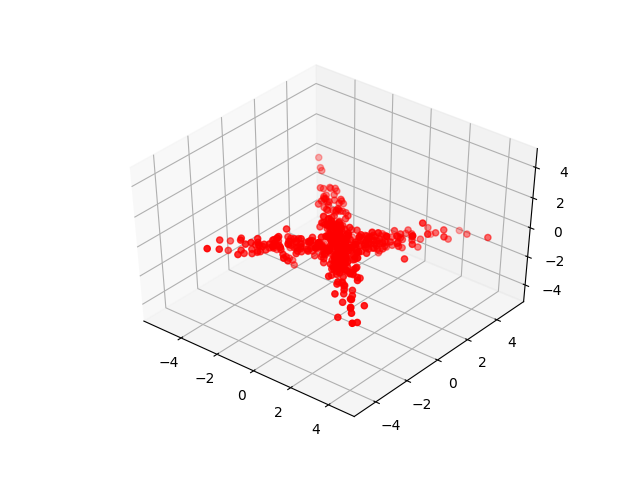
\includegraphics[width = 0.45\textwidth]{Figures/GPCA_true.png}
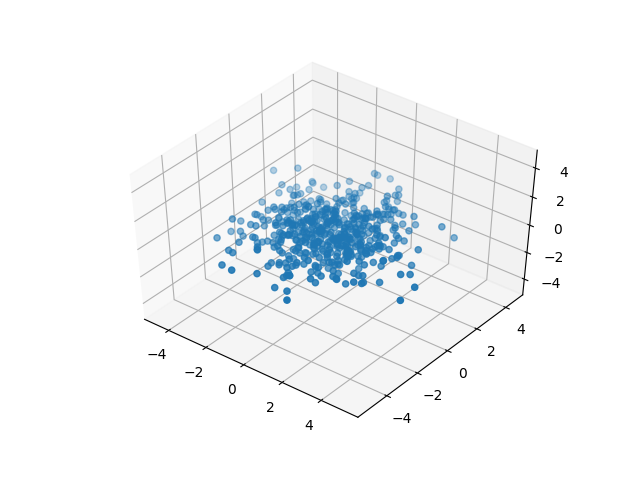
\includegraphics[width = 0.45\textwidth]{Figures/GPCA_PCA.png}
\end{center}
\caption{\label{fig:gpca} PCA cannot distinguish between the situations depicted in the two datasets.}
\end{figure} 

For simplicity, assume that we are trying to decompose the data  along unions of  hyperplanes in $\mR^d$.  Such
hyperplanes have equations of the form
$u^T\tilde x = 0$ where $\tilde x$ is our notation for the vector $(1,
x^T)^T$. If we have two hyperplanes, specified by $u_1$ and $u_2$ and all the
training samples approximately  belong to one of them, then one has, for all $k=1, \ldots, N$:
$$
(u^T_1\tx_k)(u^T_2\tx_k) = \tx_k^T u_1u_2^T \tx_k \simeq 0.
$$
Similarly, for $n$ hyperplanes, the identity is, for $k=1, \ldots, N$:
$$
\prod_{j=1}^n (u^T_j \tx_k) \simeq 0.
$$

Write
$$
\prod_{j=1}^n (u^T_j x) = \sum_{1\leq i_1, \ldots,  i_n \leq
d} u_1(i_1) \cdots u_n(i_n) x^{(i_1)}\cdots x^{(i_n)}
$$
in the form (by regrouping the terms associated with the same powers of $x$)
\begin{equation}
\label{eq:F}
F(x) = \sum_{p_1 + \ldots + p_d = n} q_{p_1\ldots p_d}\,  (x^{(1)})^{p_1} \ldots
(x^{(d)})^{p_d}\,.
\end{equation}
The collection of $\binom{n+d-1}{n}$ numbers $ Q = (q_{p_1\ldots p_n}, p_1 + \cdots + p_d = n)$ takes a specific form (that we will not need to make explicit) as a function of the unknown $u_1, \ldots, u_n$, but the first step of GPCA ignores this constraint and estimates $Q$ minimizing 
$$
\sum_{k=1}^N \left(\sum_{p_1 + \ldots + p_d = n} q_{p_1\ldots p_d} \,  (x_k^{(1)})^{p_1} \ldots
(x_k^{(d)})^{p_d}\right)^2
$$
under the constraint $\sum q_{p_1 \ldots p_n}^2 = 1$ (to avoid trivial solutions). Choosing an ordering on the set of indices $(p_1, \ldots,p_d)$ such that $p_1+ \cdots p_d=n$, one can stack the coefficients in $Q$ and the monomials $ (x_k^{(1)})^{p_1} \ldots
(x_k^{(d)})^{p_d}$ to form two vectors denoted $Q$ (with some abuse of notation) and $V(x_k)$. One can then rewrite the problem of determining $Q$ as minimizing $Q^T\Sig Q$ subject to $|Q|^2 = 1$, where 
\[
\Sig = \sum_{k=1}^N V(x_k)V(x_k)^T.
\]
The solution is given by the eigenvector associated with the smallest eigenvalue of $\Sig$. If the model is exact, this eigenvalue should be zero, and if only one decomposition of the data in a set of distinct hyperplanes exists (i.e., if $n$ is not chosen too large), then $Q$ is the unique solution up to a multiplicative constant. 

Once $Q$ is found, it remains to identify the vectors $u_1, \ldots, u_n$. This identification can be obtained by inspecting the gradient of $F$ on the union of hyperplanes. Indeed, one has, for $x\in \mR^d$,
\[
\nabla F(x) = \sum_{j=1}^n\left(\prod_{j'\neq j} u_{j'}^Tx\right) u_j
\]
However, if $x$ belong in one and only one of the hyperplanes, say $x^Tu_j = 0$, then all terms in the sum vanish but one and $\nabla F(x)$ is proportional to $u_j$. So, if the model is exact, one has, for each $k=1, \ldots, N$, either $\nabla F(x_k) = 0$ (if $x_k$ belongs to the intersection of two hyperplanes) or $\nabla F(x_k)/|\nabla F(x_k)| = \pm u_j$ for some $j$, and the sign ambiguity can be removed by ensuring, for example, that the first non-vanishing coordinate of  $u_j$ is positive. (The gradient of $F$ can be computed from $Q$ using \cref{eq:F}.) The computation of $\nabla F$ on training data therefore allows for an exact computation of the hyperplanes.


In practice, when noise is present, one cannot expect this computation to be exact.
The vectors $u_1, \ldots, u_n$ can be estimated by clustering the collection of non-vanishing gradients $\nabla F(x_k)$, $k=1, \ldots, N$. For example, one can compute a dissimilarity matrix such as  
 $d_{kl} = 1 - \cos^2(\th_{kl})$, where
$\th_{kl}$ is the angle between $\nabla F(x_k)$ and $\nabla F(x_l)$, and apply one of the methds discussed in   \cref{sec:spectral.clus}.



This analysis provides a decomposition of the training set into $n$
(or fewer) hyperplanes. The computation can then
be recursively refined in order to obtain smaller dimensional subspaces by applying the same method separately to each
hyperplane.

\section{Nuclear norm minimization and robust PCA}
\label{sec:rpca}

\subsection{Low-rank approximation}
One can also interpret PCA in terms of low-rank matrix approximations. Let $\CX_c$ be the $N$ by $d$ matrix $(x_1- \bx, \ldots, x_N-\bx)^T$, which, in generic situations, has rank $d-1$. Then PCA with $p$ components is equivalent to minimizing, over all $N$ by $d$ matrices $\CZ$ of rank $p$, the norm of the difference
\begin{equation}
\label{eq:low.rank.pca}
|\CX_c - \CZ|^2 = \trace((\CX_c-\CZ)^T(\CX_c-\CZ))\,.
\end{equation}
The quantity $|A|^2 = \trace(A^TA)$ is the sum of square of the entries of $A$, which is often referred to as the (squared) Frobenius norm. We have
\[
|A|^2 = \sum_{k=1}^d \sig_k^2
\]
where $\sigma_1, \ldots, \sigma_d$ are the singular values of $A$, i.e., the square roots of the eigenvalues of $A^TA$.

We first note the following characterization of rank-$p$ matrices.
\begin{proposition}
\label{prop.rank.p}
A matrix $\CZ$ has rank $p$ if and only if it can be written in the form $\CZ  = AW^T$ where $A$ is $N\times p$, and $W$ is $d\times p$ with $W^TW = \Id[p]$, i.e., $W = [e_1, \ldots, e_p]$ where the columns form an orthonormal family of $\mR^d$.
\end{proposition}
\begin{proof}
The ``if'' part is obvious and we prove the ``only if'' part. Assume that $\CZ$ has rank $p$.
Take  $W = [e_1, \ldots, e_p]$, where $(e_1, \ldots, e_p)$ is an orthonormal family in $\mathrm{Null}(\CZ)^\perp$. Letting $e_{p+1}, \ldots, e_d$ denote an orthonormal basis of  $\mathrm{Null}(\CZ)$, we have $\sum_{i=1}^d e_ie_i^T = \Id[d]$ and
\[
\CZ = \CZ\sum_{i=1}^d e_ie_i^T = \CZ\sum_{i=1}^p e_ie_i^T = \CZ WW^T
\]
so that one can take $A = \CZ W$. 
\end{proof}

Using this representation and letting $z_k^T$ be the $k$th row vector of $\CZ$, we have
\[
|\CX_x - \CZ|^2 = \sum_{k=1}^N |x_k - \bx -z_k|^2 = \sum_{k=1}^N \Big| x_k - \bx - \sum_{j=1}^p \pe{a_{k}} j e_j\Big|^2\,.
\]
With fixed $e_1, \ldots, e_p$, the optimal matrix $A$ has coefficients $\pe {a_{k}} j = (x_k-\bx)^Te_j$. In matrix form, this is:
\[
\CZ = \CX_c \left(\sum_{j=1}^p e_je_j^T\right).
\]


We therefore retrieve the PCA formulation that we gave in  \cref{sec:pca}, in the special case of $H = \mR^d$ with the standard Euclidean product.  The lowest value achieved by the PCA solution is 
\[
|\CX_c - \CZ|^2 = N\sum_{k=p+1}^d \la_k^2
\]
where $\la_1^2, \ldots, \la_d^2$ are the eigenvalues of the covariance matrix computed from $x_1, \ldots, x_N$, who are also the squared singular values of the matrix $\CX_c$ divided by $N$.

In this section, we will explore variations on PCA in which the minimization of  $|\CX_c - \CZ|^2$ is completed with a penalty that depends on the singular values of the matrix $\CZ$. As a first example, 
one can modify PCA by adding  a penalty on the rank (i.e., on the number of non-zero singular values), minimizing:
\[
{\ga} |\CX_c - \CZ|^2+  \rank(\CZ)
\]
for some parameter $\ga>0$. However, the solution to this problem is a small variation of that of standard PCA. It is indeed given  by standard PCA with $p$ components where $p$ minimizes 
\[
N\ga \sum_{k=p+1}^d \la_k^2 +  p = N\ga \sum_{k=p+1}^d (\la_k^2 - (N\ga)^{-1}) + d,
\]
i.e.,  $p$ is the index of the last eigenvalue that is larger than $(N\ga)^{-1}$.

\subsection{The nuclear norm}
Based on the fact that $\rank(\CZ)$ is the number of non-zero singular values of $\CZ$, one can use the same heuristic as in the development of the lasso, and replace  counting the non-zero values by the sum of the absolute values of the singular values, which is just the sum of singular values since they  are non-negative. This provides the nuclear norm of $A$, defined in \cref{sec:matrix.norms} by
\[
|A|_* = \sum_{k=1}^d \sig_k
\]
where $\sigma_1, \ldots, \sigma_d$ are the singular values of $A$.  We will consider below the problem of minimizing
\begin{equation}
\label{eq:robust.pca.2}
{\ga} |\CX_c - \CZ|^2+  |\CZ|_*
\end{equation}
and show that its solution is once again similar to PCA.

We recall the characterization of the nuclear norm \cref{prop:nuclear}. If $A$ is an  $N$ by $d$ matrix,
\[
|A|_* = \max\Big\{\trace(UAV^T): U \text{ is }N\times N \text{ and } U^TU = \Id,  V \text{ is } d\times d \text{ and } V^TV = \Id\Big\}\,.
\]

In \citet{cai2010singular}, the authors consider the minimization of \cref{eq:robust.pca.2} 
and prove the following result. Recall that we have defined the shrinkage function $S_\tau: t \mapsto \sign(t)\max(|t|-\tau, 0)$ (with $\tau \geq 0$), using the same notation $S_\tau(X)$ when applying $S_\tau$ to every entry of a vector or matrix $X$.   Following \citet{cai2010singular}, we define the {\em singular value thresholding operator} $A \mapsto \mS_\tau(A)$, where $A$ is any rectangular matrix, by
\[
\mS_\tau(A) = US_\tau(\Delta) V^T
\]
when $A = U\Delta V^T$ is a singular value decomposition of $A$.
\begin{proposition}
\label{prop:sh.svd}
Let us assume without loss of generality that $N\geq d$. 
The function $\CZ \mapsto {\ga} |\CX_c - \CZ|^2+  |\CZ|_*$ is minimized by $\CZ = \mS_{1/2\ga}(\CX)$.
\end{proposition}
\begin{proof}
Representing $\CZ$ by its singular value decomposition, we have the equivalent formulation of minimizing 
\begin{align*}
F(U, V, D) &= \ga|\CX_c - UDV^T|^2 +  |D|_*\\
&= \ga|\CX_c|^2 - 2\ga\trace(\CX_c^TUDV^T) + \ga|D|^2 + |D|_*
\end{align*}
over all orthonormal matrices $U$ and $V$ and diagonal matrices with non-negative coefficients $D$. From \cref{th:trace.ineq}, we know that $\trace(\CX_c^TUDV^T)$ is less than the sum of the products of the non-increasingly ordered singular values of $\CX_c$ and $D$ and this upper bound is attained by taking $U= \bar U$ and $V=\bar V$ where $\bar U$ and $\bar V$ are  the matrices providing the SVD of $\CX_c$, i.e., such that $\CX_c = \bar U\Delta \bar V^T$ where $\Delta$ is diagonal with non-decreasing coefficients along the diagonal. So, letting $\la_1 \geq \cdots \geq \la_d \geq 0$ and $\mu_1 \geq \cdots \geq \mu_d\geq 0$ be the singular values of $\CX_c$ and $\CZ$, we have just proved that, for any $D$,
\[
F(U, V, D) \geq  F(\bar U, \bar V, D) = -2\ga \sum_{i=1}^d \mu_i\la_i + \ga\sum_{i=1}^d \mu_i^2 + \sum_{i=1}^d\mu_i\,.
\]
The lower bound is minimized when  $\mu_i = \max(\la_i - 1/2\ga, 0)$. This proves the proposition.
\end{proof}



\subsection{Robust PCA}
As a consequence, the nuclear norm penalty provides the same principal directions (after replacing $\ga$ by $2\ga$) as the rank penalty, but applies a shrinking operation rather than thresholding on the singular values. The difference is however more fundamental if, in addition to using the nuclear norm as a penalty, on replaces the squared Frobenius norm on the approximation error by the $\ell^1$ norm, where, for an $n$ by $m$ matrix $A$ with coefficients $(a(i,j))$,
\[
|A|_{\ell_1} = \sum_{i,j} |a(i,j)|\,.
\]
This is the formulation of  robust PCA \citep{candes2011robust}, which minimizes
\begin{equation}
\label{eq:r.pca}
{\ga} |\CX_c - \CZ|_{\ell^1}+  |\CZ|_*
\end{equation}
with respect to $\CZ$.

Robust PCA (which was initially named Principal Component Pursuit by the authors in \citet{candes2011robust}) is designed for situations in which $\CX_c$ can be decomposed as the sum of a low-rank matrix $\CZ$ and of a sparse residual $S$. Some theoretical justification was provided in the original paper, stating that if $\CX_c = \CZ + S$, with $\CZ = UDV^T$ (its singular value decomposition) such that $U$ and $V$ are sufficiently ``diffuse'' and $\rank(\CZ)$ is small enough, with the residual's sparsity pattern taken uniformly at random over the subsets of entries of $S$ with a sufficiently  small cardinality, then robust PCA is able to reconstruct the decomposition exactly with high probability (relative to the random selection of the sparsity pattern of $S$). We refer to \citet{candes2011robust} for the long proof that justifies this statement.

Robust PCA can be solved using the ADMM algorithm (\cref{sec:proximal}) after reformulating the problem as the minimization of 
\[
\ga |R|_{\ell_1} +  |\CZ|_*
\]
subject to $R + \CZ = \CX_c$.  The algorithm therefore iterates over the following steps.
\begin{equation}
\label{eq:pcp}
\left\{
\begin{aligned}
\CZ^{(k+1)} &=  \argmin_\CZ \Big( |\CZ|_* + \frac{1}{2\al} |\CZ + R^{(k)} - \CX_x + U^{(k)}|^2\Big)\\
R^{(k+1)} &= \argmin_R \Big(\ga |R|_{\ell^1} + \frac1{2\al} |\CZ^{(k+1)} + R - \CX_c + U^{(k)}|^2\Big) \\
U^{(k+1)} &= U^{(k)} + \CZ^{(k+1)} + R^{(k+1)} - \CX_c
\end{aligned}
\right.
\end{equation} 
The first minimization is covered by  \cref{prop:nuclear} and yields
\[
\CZ^{(k+1)} = \mS_\al(\CX_c - R^{(k)} - U^{(k)}).
\]
The second minimization is solved by a standard shrinking operation, i.e., 
\[
R^{(k+1)} = S_{\ga\al} (\CX_c - \CZ^{(k+1)} - U^{(k)}). 
\]
Using this, we can rewrite the robust PCA algorithm as the sequence of fairly simple iterations.
\begin{algorithm}
\label{alg:robust.pca}
\begin{enumerate}
\item Choose a small enough constant $\alpha$ and a very small tolerance level $\epsilon$.
\item Initialize the algorithm with $N$ by $d$ matrices $R^{(0)}$ and $U^{(0)}$ (e.g., equal to zero).
\item At step $n$, apply the iteration: 
\begin{equation}
\label{eq:pcp.2}
\left\{
\begin{aligned}
\CZ^{(k+1)} &= \mS_\al(\CX_c - R^{(k)} - U^{(k)}) \\
R^{(k+1)} &=S_{\ga\al} (\CX_c - \CZ^{(k+1)} - U^{(k)}) \\
U^{(k+1)} &= U^{(k)} + \CZ^{(k+1)} + R^{(k+1)} - \CX_c
\end{aligned}
\right.
\end{equation} 
\item Stop the algorithm is the variation compared to variables at the previous step is below the tolerance level. Otherwise, apply step $n+1$.
\end{enumerate}
\end{algorithm}


\section{Independent component analysis}


%Independent component analysis adopts a strategy very different from PCA. 
Independent component analysis (ICA) is a factor analysis method that represents  a $d$-dimensional random variable $X$  in the form
$X = A Y$ where $A$ is a fixed $d\ti d$ invertible matrix and
$Y$ is a $d$-dimensional random vector with independent components. 
There are two main approaches in this setting. The first one optimizes the matrix $W = A^{-1}$ so that  the components of $WX$ are ``as independent as possible'' according to a suitable criterion. The second one is  model-based, where a statistical model is assumed for $Y$, and its parameters, together with the entries of the matrix $A$, are estimated via maximum likelihood. Before describing each of these methods, we first discuss the extent to which the coefficients of $A$ are identifiable. 

\subsection{Identifiability}

A statistical model is identifiable if its parameters (which could be finite- of infinite-dimensional) are uniquely defined by the distribution of the observable variables. In the case of ICA, this question boils down to deciding whether $AY \sim A'Y'$ (i.e., they have the same probability distribution) implies that $A = A'$ (where $Y$ and $Y'$ are two random vectors with independent components).

It should be clear that the answer to this question is negative, because there are trivial transformations of the matrix $A$ that do not break the ICA model. One can, for example, take any invertible diagonal matrix, $D$, and let $A' = AD^{-1}$ and $Y' = DY$. The same statement can be made if $D$ is replaced by a permutation matrix, $P$, which reorders the components of $Y$. So we know that $AY \sim A'Y'$ is possible already when $A' = ADP$ where $D$ is diagonal and invertible and $P$ is a permutation matrix. Note that iterating such matrices (i.e., letting $A' = ADPD'P'$) does not extend the class of transformations because one  has $DP = PP^{-1}DP$ and one can easily check that  $P^{-1}DP$ is diagonal, so that one can rewrite any product of permutations and diagonal matrices as a single diagonal matrix multiplied by a single permutation. 

It is interesting, and fundamental for the well-posedness of ICA, that, under one  important additional assumption, the indeterminacy in the identification of $A$ stops at these transformations. The additional assumption is that at most one of the components of $Y$ follows a Gaussian distribution. That such a restriction is needed is clear from the fact that one can transform any Gaussian vector $Y$ with independent components into another, $BY$, one as soon as $BB^T$ is diagonal. If two or more components of $Y$ are Gaussian, one can restrict these matrices $B$ to only affect those components. If only one of them is Gaussian, such an operation has no effect. 

The following theorem is formally stated in \citet{comon1994independent}, and is a rephrasing of the Darmois-Skitovitch theorem \citep{darmois1953analyse,skitovich1954linear}. The proof of this theorem relies on complex analysis arguments on characteristic functions and is beyond the scope of these notes (see \citet{kagan1973characterization} for more details).

\begin{theorem}
\label{th:ica.charac}
Assume that $Y$ is a random vector with independent components, such that at most one of its components is Gaussian. Let $A$ be an invertible linear transformation and $\tilde Y = CY$. Then the following statements are independent. 
\begin{enumerate}[label=(\roman*)]
\item For all $i\neq j$, the components $\pe{\tilde Y} i , \tilde Y^{(j)}$ are independent.
\item $\tilde Y^{(1)}, \ldots, \tilde Y^{(d)}$ are mutually independent. 
\item $C = DP$ is the product on a diagonal matrix and of a permutation.
\end{enumerate}
\end{theorem}

The equivalence of (ii) and (iii) implies that the ICA model is identifiable up to multiplication on the right by a permutation and a diagonal matrix. Indeed, if $X = AY = A'Y'$ are two decompositions, then it suffices to apply the theorem  to $C = (A')^{-1} A$ to conclude. The equivalence of (i) and (ii) is striking, and has the important consequence that, if the data satisfies the ICA model, then, in order to identify $A$ (up to the listed indeterminacy), it suffices to look for $Y = A^{-1}X$ with pairwise independent components, which is a much lesser constraint than full mutual independence. 

As a final remark on the Gaussian indeterminacy, we point out that, if the mean ($m$) and covariance matrix ($\Sig$) of $X$ are known (or estimated from data), the ICA problem can be reduced to looking for orthogonal transformations $A$. Indeed, assuming $X = AY$ and letting $\tX = \Sig^{-1/2} (X - m)$ and $\tY = D^{-1/2}(Y - A^{-1} m)$, where $D$ is the (diagonal) covariance matrix of $Y$, we have
\[
\tX = \Sig^{-1/2}(AY - m) = \Sig^{-1/2}A D^{1/2} \tY.
\]
Letting $\tilde A = \Sig^{-1/2}A D^{1/2}$, we have $\Id_{\mR^d} = E(\tX \tX^T) = \tilde A \tilde A^T$ so that $\tilde A$ is orthogonal. This shows that  the ICA problem for $\tX$ in the form $\tX = \tilde A \tY$ with the restriction that $\tilde A$ is orthogonal has a solution, and also provides a solution of the original ICA problem by letting $A = \Sig^{1/2} \tilde A$ and $Y = \tY - \tilde A^{-1} \Sig^{-1/2} m$. Therefore, the indeterminacy associated with Gaussian vectors is as general as possible up to a normalization of first and second moments.

\subsection{Measuring independence and non-Gaussianity}

Independence between $d$ variables is a very strong property and its complete characterization is computationally challenging. The fact that the joint p.d.f.of the $d$ variables  (we will restrict, to simplify our discussion, to variables that are absolutely continuous) factorizes into the product of the marginal p.d.f.'s of each variable can be measured by computing the mutual information between the variables, defined by (letting $\phi_Z$ denote the p.d.f. of a variable $Z$)
\[
I(Y) = \int \frac{\phi_Y(y)}{\prod_{i=1}^d \phi_{\pe Y i}(\pe y i)} \phi_Y(y) dy.
\]
The mutual information is always non-negative and vanishes only if the components of $Y$ are mutually independent.
Therefore, one can represent ICA as an optimization problem minimizing $I(WX)$ with respect to all invertible matrices $W$ (so that $W = A^{-1}$). Letting
\[
h(Y) = - \int \log \phi_Y(y)\, \phi_Y(y) dy
\]
denote the ``differential entropy'' of $Y$, we can write
\[
I(Y) = \sum_{i=1}^d h(\pe Y i) - h(Y).
\]

If $Z = WX$, then $\phi_Z(z) = \phi_X(W^{-1}x) |\det(W)|^{-1}$. Using this expression in $h(Z)$ and making a change of variables yields $h(WZ) = h(X) + \log |\det W|$ and 
\[
I(WX) = \sum_{i=1}^d h(\pe Z i) - \log |\det(W)| - h(X).
\]
This shows that the optimal $W$ can be obtained by minimizing
\[
F(W) =  \sum_{i=1}^d h(W^{(i)}X) - \log |\det(W)|
\]
where $W^{(i)}$ is the $i$th row of $W$. This brings a notable simplification, since this expression only involves differential entropies of scalar variables, but still remains a  challenging problem. 

In \citet{comon1994independent}, it is proposed to use cumulant expansions of the entropy around that of a Gaussian with identical mean and variance to approximate the differential entropy. If $\xi \sim \CN(m, \sig^2)$ , then
\[
h(\xi) = \frac12 + \frac12 \log(2\pi\sig^2).
\]
Define, for a general random variable $U$ with standard deviation $\sigma_U$, the non-Gaussian entropy, or negentropy, defined by 
\[
\nu(U) = \frac12 + \frac12 \log(2\pi\sig_U^2) - h(U)\,.
\]
One can shows that $\nu(U) \geq 0$ and is equal to 0 if and only if $U$ is Gaussian. One can rewrite $F(W)$ as 
\[
F(W) =  \frac d2 + \frac d2 \log(2\pi) + \sum_{i=1}^d \log(\sig_{W^{(i)}X}^2) - \sum_{i=1}^d \nu(W^{(i)}X) - \log |\det(W)|
\]

As we remarked earlier, if we replace $X$ by $\Sig^{-1/2} (X-m)$ (after estimating the covariance matrix of $X$), there is no loss of generality in requiring that $W$ is an orthogonal matrix, in which case both $\sig_{W^{(i)}X}^2$ and $|\det W|$ are equal to 1. Assuming such a reduction is done, we see that the problem now requires to maximize
\begin{equation}
\label{eq:negentropy}
\sum_{i=1}^d \nu(W^{(i)}X)
\end{equation}
among all orthogonal matrices $W$. Still in \citet{comon1994independent}, an approximation of the negentropy $\nu(U)$ is provided as a function of the third and fourth cumulants of the distribution of $U$. These are given by
\[
\ka_3 = E((U-E(U))^3)
\]
and
\[
\ka_4 = E((U-E(U))^4) - 3\sig_U^4.
\]
In particular, when $U$ is normalized, i.e.,  $E(U) = 0$ and $\sig^2_U = 1$, we have $\ka_3 = E(U^3)$ and $\ka_4 = E(U^4) - 3$. Under the same assumption, it is proposed in \citet{comon1994independent} to use the approximation
\[
\nu(U) \sim \frac{\ka_3^2}{12} + \frac{\ka_4^2}{48} + \frac{7\ka_3^4}{48} - \frac{\ka_3^2\ka_4}{8}\,.
\]
This approximation was derived from an Edgeworth expansion of the p.d.f. of $U$, which can be seen as a Taylor expansion around a Gaussian distribution. Plugging this expression into \cref{eq:negentropy} provides an expression that can be maximized in $W$ where the cumulants are replaced by their sample estimates. However, the maximized function involves high-degree polynomials in the unknown coefficients of $W$, and this simplified problem still presents numerical challenges. 

\bigskip

An alternative approximation of the negentropy has been proposed in \citet{hyvarinen1998new} relying on the maximum entropy principle, described in the following theorem. Associate to any random variable $Y:\CG \to \mR$ the differential entropy
\[
h_\mu(Y) = - \int_{\CG} \log \phi_Y(x) \phi_Y(x) d\mu(x)
\]
if the distribution of $Y$ has a density, denoted $\phi_Y$, with respect to $\mu$ and $h_\mu(Y) = -\infty$ otherwise.
Use also the same notation
\[
h_\mu(\phi) = - \int_{\CG} \log \phi(x) \phi(x) d\mu(x)
\]
for a p.d.f. $\phi$ with respect to $\mu$ (i.e., such that $\phi$ is non-negative and has integral 1). Then, the following is true.
\begin{theorem}
\label{th:max.ent.principle}
Let $\bfg = (\pe g 1, \ldots, \pe g p)^T$ be a function defined on a measurable space $\CG$, taking values in $\mR^p$, and let $\mu$ be a measure on $\CG$. Let $\Gamma_\mu$ be the set of all   
$\boldsymbol\lambda = (\pe \lambda 1, \ldots, \pe \lambda p)\in \mR^p$ such that 
\begin{equation}
\label{eq:max.ent.principle.2}
\int_\CG \exp\left(\boldsymbol\la^T \bfg(y)\right) d\mu(y) < \infty.
\end{equation}
Then 
\begin{equation}
\label{eq:max.ent.principle.0}
h_\mu(Y) \leq \mathrm{inf}\left\{- \boldsymbol\la^T E(\bfg(Y)) + \log \int_\CG \exp\left(\boldsymbol\la^T \bfg(y)\right) d\mu(y): \boldsymbol\lambda \in \Gamma_\mu \right\}.
\end{equation}


Define, for $\boldsymbol\lambda\in \Gamma_\mu$, 
\begin{equation}
\label{eq:max.ent.exp}
\psi_{\boldsymbol \lambda}(x) = \frac{\exp\left(\boldsymbol\la^T \bfg(x)\right) d\mu(x)}{\int_\CG \exp\left(\boldsymbol\la^T \bfg(y)\right) d\mu(y)}.
\end{equation}

Assume that the infimum in \cref{eq:max.ent.principle.0} is attained at an interior point $\boldsymbol \lambda^*$ of $\Gamma_\mu$. Then 
\begin{equation}
\label{eq:max.ent.principle.3}
h(\phi_{\boldsymbol\lambda^*}) = \max\{h(\tilde Y): E_{\tilde Y}(\bfg) = E_Y(\bfg), i=1, \ldots, p\}.
\end{equation}
\end{theorem}

\begin{proof}


Let $Y$ be a random variable with p.d.f. $\phi_Y$ with respect to $\mu$ (otherwise the lower bound in \cref{eq:max.ent.principle.0} is $-\infty$). 
Then
\[
h_\mu(Y) + \boldsymbol\la E(\bfg(Y)) - \log \int \exp\left(\boldsymbol\la \bfg(y)\right) d\mu(y) = - \int_\CG \phi_Y(x) \log \frac{\phi_Y(x)}{\psi_{\boldsymbol\lambda}(x)} d\mu(x) \leq 0
\]
since $\int_\CG \phi_Y(x) \log \frac{\phi_Y(x)}{\psi_{\boldsymbol\lambda}(x)} d\mu(x)$ is a KL divergence and is always non-negative.

Assume that $\boldsymbol\lambda$ is in $\mathring \Gamma_\mu$. Then, there exists $\epsilon > 0$ such that, for any $\bfu\in \mR^p$, $|\bfu|=1$, $\boldsymbol\lambda + \epsilon \bfu\in \Gamma_\mu$. Using the fact that $e^\beta \geq e^\alpha + (\beta-\alpha)e^\alpha$, we can write
\begin{align*}
\epsilon \bfu^T \bfg e^{\lambda^T \bfg} &\leq e^{(\lambda+\epsilon u)^T\bfg} - e^{\lambda^T \bfg}\\
-\epsilon \bfu^T \bfg e^{\lambda^T \bfg} &\leq e^{(\lambda-\epsilon u)^T\bfg} - e^{\lambda^T \bfg}
\end{align*}
yielding
\[
\epsilon |\bfu^T \bfg| e^{\lambda^T \bfg} \leq \max(e^{(\lambda+\epsilon u)^T\bfg}, e^{(\lambda-\epsilon u)^T\bfg}) - e^{\lambda^T \bfg} \leq e^{(\lambda+\epsilon u)^T\bfg} + e^{(\lambda-\epsilon u)^T\bfg} - e^{\lambda^T \bfg}.
\]
Since the upper-bound is integrable with respect to $\mu$, so is the lower bound, showing that (taking $\boldsymbol u$ in the canonical basis of $\mR^p$)
\[
\int_\CG |\pe g i(y)| e^{\lambda^T \bfg(y)}d\mu(y) <\infty
\]
for all $i$, or
\[
\int_\CG |\boldsymbol g(y)| e^{\lambda^T \bfg(y)}d\mu(y) <\infty.
\]
Let $\bfc = E(\bfg(Y))$ and define
\begin{equation}
\Psi_{\boldsymbol c}(\boldsymbol\la) = - {\boldsymbol c}^T\boldsymbol\la +  \log \int \exp(\boldsymbol\la^T\boldsymbol g(y)) dy.
\label{eq:max.ent.psi}
\end{equation} 
Then
\[
\prt_{\boldsymbol\lambda} \Psi_c = - c^T + \frac{\int \boldsymbol g(x)^T\exp(\boldsymbol\la^T\boldsymbol g(x)) dx}{\int \exp(\boldsymbol\la^T\boldsymbol g(y)) dy}
= -c^T + \int_{\CG} \boldsymbol g(x)^T \psi_{\boldsymbol\lambda}(x) dx\,.
\]
Since $\boldsymbol \la^*$ is a minimizer, we find that,  if $\tilde Y$ is a random variable with p.d.f. $\boldsymbol\lambda^*$, then $E(\tilde Y) = c = E(Y)$. In that case, the upper-bound in \cref{eq:max.ent.principle.0} is $h_\mu(\tilde Y)$, proving \cref{eq:max.ent.principle.3}.
\end{proof}
\begin{remark}
The previous theorem is typically applied with $\mu$ equal to Lebesgue's measure on $\CG = \mR^d$ or to a counting measure with $\CG$  finite. To rewrite the statement of \cref{th:max.ent.principle} in those cases, it suffices to replace $d\mu(x)$ by $dx$ for the former, and integrals by sums over $\CG$ for the latter. In the rest of the discussion, we restrict to the case when $\mu$ is Lebesgue's measure,  using $h(Y)$ instead of $h_\mu(Y)$.
\end{remark}

\begin{remark}
This principle justifies, in particular, that the negentropy is always non-negative since it implies that a distribution that maximizes the entropy given its first and second moments must be Gaussian.  
\end{remark}

The right-hand side of \cref{eq:max.ent.principle.0} provides a variational approximation of the entropy. If one uses this approximation when minimizing 
$h(W^{(1)} X) + \cdots + h(W^{(d)} X)$, the resulting problem can be expressed as a minimization, with respect to
$W$ and $\boldsymbol\lambda_1, \ldots, \boldsymbol\lambda_d\in \mR^p$ of
\[
- \sum_{j=1}^d \boldsymbol\la^T E(\bfg(W^{(j)}X)) + \sum_{j=1}^d \log \int \exp\left(\boldsymbol\la^T \bfg(y)\right)\,dy\,.
\]

While it would be possible to solve this optimization problem directly,  a further approximation of the upper bound can be developed leading to a simpler procedure. We have seen in the previous proof that, defining $\Psi_{\bfc} $ by \cref{eq:max.ent.psi} and denoting by  $E_{\boldsymbol\la}$ the expectation with respect to $\phi_{\boldsymbol\lambda}$, one has
\[
\nabla \Psi_\bfc(\boldsymbol\la) = - \bfc + E_{\boldsymbol\la}(\bfg)\,.
\]
Taking the second derivative, one finds
\[
\nabla^2 \Psi_\bfc(\boldsymbol\la) = E_{\boldsymbol\la}((\bfg-E_{\boldsymbol\la}(\bfg))(\bfg-E_{\boldsymbol\la}(\bfg))^T).
\]
Now choose $\bfc_{0}$ such that a maximizer of $\Psi_{\bfc_{0}}(\boldsymbol\la)$, say, $\boldsymbol\la^{\bfc_{0}}$, is known. If $\bfc$ is close to $\bfc_{0}$, a first order expansion indicates that, for $\boldsymbol\la^{\bfc}$ maximizing $\Psi_\bfc$, one should have
\[
\boldsymbol\la^{\bfc} \simeq \boldsymbol\la^{\bfc_{0}} + \nabla^2 \Psi_\bfc(\boldsymbol\la^{\bfc_{0}})^{-1} (\bfc - \bfc_{0})
\]
with
\[
\Psi_\bfc(\boldsymbol\la^c)\simeq \Psi_\bfc(\boldsymbol\la^{\bfc_{0}}) - (\bfc-\bfc_{0})^T\nabla^2 \Psi_\bfc(\boldsymbol\la^{\bfc_{0}})^{-1} (\bfc - \bfc_{0}). 
\]
One can then use the right-hand side as an approximation of the optimal entropy. 

This leads to simple computations under the following assumptions. First, assume that  the first two functions $\pe g1$ and $\pe g2$ are $u$ and $u^2/\sqrt 3$. 
Let $\phi_0$ be the p.d.f. of a standard Gaussian. Assume that the functions $\pe g j$ are chosen so that
\[
\int \pe g i(u) \pe g j(u) \phi_0(y) dy = \de_{ij}
\]
for $i,j=1, \ldots, p$ and such that $\int \pe g i(u) \phi_0(y) dy = 0$ for $i\neq 2$. Take
\[
\bfc_0 = \int \bfg \phi_0(u) du
\]
so that $c^{(1)}_0=0$, $c^{(2)}_0 = 1/\sqrt 3$ and $c^{(i)}_0 = 0$ for $i\geq 2$.

Then $\la^{\bfc_{0}}$ provides, by construction, the distribution $\phi_0$ and  for any $\bfc$, $\nabla^2\Psi_\bfc(\boldsymbol\la^{\bfc_{0}}) = \Id[p]$. With these assumptions, the approximation is 
\begin{align*}
\Psi_\bfc(\boldsymbol\la) &= h(\phi_0) - |\bfc-\bfc_{0}|^2\\
&= \frac12(1+ \log 2\pi) - \sum_{j\geq 3} (\pe c j)^2 
\end{align*}
(assuming that the data is centered and normalized so that $\pe c 1 = 0$ and $\pe c 2 = 1/\sqrt 3$). The ICA problem can then be solved by maximizing
\begin{equation}
\label{eq:ica.easy}
\sum_{j=1}^d \sum_{i=1}^p E(\pe g i(W^{(j)} X))^2
\end{equation}
over orthogonal matrices $W$. 

\begin{remark}
Without the assumption made on the functions $\pe g j$, one needs to compute $S = \Cov(g(U))^{-1}$ where $U\sim \CN(0,1)$ and maximize
\[
\sum_{j=1}^d (E(\bfg(W^{(j)} X)) - E(\bfg(U)))^TS(E(\bfg(W^{(j)} X)) - E(\bfg(U))).
\]
Clearly, this expression can be reduced to \cref{eq:ica.easy} by replacing $\bfg$ by $S^{-1/2}(\bfg- E(\bfg(U)))$. Note also that we retrieve here a similar idea to the negentropy, maximizing a deviation to a Gaussian.
\end{remark}

\subsection{Maximization over orthogonal matrices}
\label{sec:grad.orthogonal}
In the previous discussion, we reached a few times a formulation of ICA which required optimizing a function $W \mapsto F(W)$ over all orthogonal matrices. We now discuss how such a problem may be implemented. 

In all the examples that were considered, there would have been no loss of generality in requiring that $W$ is a rotation, i.e., $\det(W) = 1$. This is because one can change the sign of this determinant by simply changing the sign of one of the independent components, which is always possible. (In fact, the indeterminacy in $W$ is by right multiplication by the product of a permutation matrix and a diagonal matrix with $\pm1$ entries.)

Let us assume that $F(W)$ is actually defined and differentiable over all invertible matrices, which form an open subset of the linear space $\CM_d(\mR)$ of $d$ by $d$ matrices.  Our optimization problem can therefore be considered as the minimization of $F$ with the constraint that $WW^T = \Id[d]$. 

Gradient descent derives from the analysis that a direction of descent should be a matrix $H$ such that $F(W + \ep H) < F(W)$ for small enough $\ep>0$ and on the remark that $H = -\nabla F(W)$ provides such a direction. This analysis does not apply to the constrained optimization setting because, unless the constraints are linear, $W+\ep H$ will generally stop to satisfy the constraint when $\ep >0$, requiring the use of more complex procedures. In our case, however, one can take advantage of the fact that orthogonal matrices form a group to replace the perturbation $W \mapsto W + \ep H$ by $W \mapsto We^{\ep H}$ (using the matrix exponential) where $H$ is moreover required to be skew symmetric ($H+H^T=0)$, which guarantees that $e^{\ep H}$ is an orthogonal matrix with determinant 1. Now, using the fact that $e^{\ep H} = \Id + \ep H + o(\ep)$, we can write
\[
F(We^{\ep H}) = F(W) + \ep \trace(\nabla F(W)^T WH) + o(\ep)\,.
\]
Let $\nabla^s F(W)$ be the skew symmetric part of $W^T\nabla F(W)$, i.e., 
\[
\nabla^s F(W) = \frac12 (W^T\nabla F(W) - \nabla F(W)^TW).
\]
Then, if $H$ is skew symmetric, 
\begin{align*}
\trace(\nabla^s F(W)^T H) &= \frac12 \trace(\nabla F(W)^T WH) - \frac12 \trace(W^T\nabla F(W) H) \\
&=  \frac12 \trace(\nabla F(W)^T WH) + \frac12 \trace(W^T\nabla F(W) H^T)\\
& = \trace(\nabla F(W)^T WH) 
\end{align*}
so that 
\[
F(We^{\ep H}) = F(W) + \ep \trace(\nabla^s F(W)^T H) + o(\ep)\,.
\]
This show that $H = - \nabla^s F(W)$ provides a direction of descent in the orthogonal group, in the sense that, if $\nabla^s F(W) \neq 0$, 
\[
F(We^{-\ep\nabla^s F(W)}) < F(W)
\]
for small enough $\ep > 0$. As a consequence, the algorithm 
\[
W_{n+1} = W_n  e^{-\ep_n\nabla^s F(W_n)}
\]
combined with a line search for $\ep_n$ implements gradient descent in the group of orthogonal matrices, and therefore converges to a local minimizer of $F$. 

If one linearizes the r.h.s. as a function of $\ep$, one gets
\begin{align*}
W_n  e^{-\ep_n\nabla^s F(W_n)} &=  W_n + \frac{\ep_n} 2 W_n( (W_n)^T\nabla F(W_n) - \nabla F(W_n)^TW_n) + o(\ep)\\
& = W_n + \frac{\ep_n} 2 ( \nabla F(W_n) - W_n\nabla F(W_n)^TW_n) + o(\ep).
\end{align*}
As already argued, this linearized version cannot be used when optimizing over the orthogonal group. However, if one denotes by $\om(A)$ the unitary part of the polar decomposition of $A$, i.e., $\om(A) = (AA^T)^{-1/2}A$, then the algorithm
\[
W_{n+1} = \om\left(W_n + \frac{\ep_n} 2 ( \nabla F(W_n) - W_n\nabla F(W_n)^TW_n)\right)
\]
also provides a valid gradient descent algorithm.
\bigskip

\subsection{Parametric ICA}
We now describe a parametric version of ICA in which a model is chosen for the independent components of $Y$. The simplest version of to assume that all $Y^{(j)}$ are i.i.d. with some prescribed p.d.f., say, $\psi$. A typical example for $\psi$ is a logistic distribution with
\[
\psi(t) = \frac{2}{(e^t+
e^{-t})^2}.
\]
If $y$ is a vector in $\mR^d$, we will use, as usual, the notation $\psi(y)  = (\psi(y^{(1)}), \ldots, \psi(y^{(d)}))^T$ for $\psi$ applied to each component of $y$.

The model parameter is then the matrix $A$, or preferably $W = A^{-1}$, and it may be estimated using maximum likelihood. Indeed, the p.d.f. of $X$ is
$$
f_X(x) = |\det W|\, \prod_{j=1}^d \psi(W^{(j)}x)
$$
where $W^{(j)}$ is the $j$th row of $W$, so that $W$ can be estimated by maximizing
\[
\ell(W) = N \log\abs{\text{det}(W)} +  \sum_{k=1}^N \sum_{j=1}^d \log \psi(W^{(j)}x_k)\,.
\]
If we denote by $\Ga(W)$ the matrix with coefficients 
\[
\ga_{ij}(W) = \sum_{k=1}^N x_k(i) \frac{\psi'(W^{(j)}x_k)}{\psi(W^{(j)}x_k)}
\]
and use the fact that the gradient of $W \mapsto \log |\det W|$ is $W^{-T}$ (the inverse transpose of $W$), we can write
\[
\nabla \ell(W) = NW^{-T} + \Ga(W).
\] 

We need however the maximization to operate on sets of invertible matrices, and it is more natural to move in this set through multiplication than through addition, because the product of two invertible matrices is always invertible, but not necessarily their sum. So, similarly to the previous section, we will look for small variations in the form  $W \mapsto We^{\ep H}$, or simply, in this case, $W \mapsto W(\Id[d] + \ep H)$. In both case, the first order expansion of the log-likelihood gives
\[
\ell(W) + \ep \trace((NW^{-T} + \Ga(W))^TWH)
\]
which suggests taking 
\[
H = W^T(NW^{-T} + \Ga(W)) = N\Id + W^T\Ga(W).
\]

Dividing $H$ by $N$, we obtain the following variant of gradient ascent for maximum likelihood
\[
W_{n+1} = (1 + \ep_n) W_n +  \ep_n W_nW_n^T\Ga(W_n)\,.
\]
This algorithm numerically performs much better than standard gradient ascent. It moreover presents the advantage of avoiding computing the inverse of $W$ at each step. 


\subsection{Probabilistic ICA}

Note that the algorithms that we discussed concerning ICA were all formulated in terms of the matrix $W = A^{-1}$, which ``filters'' the data into independent components. As a result, ICA requires as many independent components 
 as the dimension of  $X$. Moreover, because the components are typically normalized to have equal variance, there is no obvious way to perform dimension reduction using this method. Indeed, ICA is typically run after the data is preprocessed using PCA, this preprocessing step providing the reduction of dimension.

It is however possible to define a model similar to probabilistic PCA, assuming a limited number of components to which a Gaussian noise is added, in the form
$$
X  = \sum_{j=1}^p a_j Y^{(j)} + \sig R 
$$
with $p< d$, $a_1, \ldots, a_p\in \mR^d$,  $Y^{(1)},
\ldots, Y^{(p)}$ independent variables as before, and $R \sim \CN(0, \Id_{\mR^d})$.  This model is identifiable (up to permutation and scalar multiplication of the components) as soon as none of the variables $Y^{(j)}$  is Gaussian.

 Let us assume a parametric setting similar to that of the previous section, so that $Y^{(1)}, \ldots, Y^{(p)}$ are explicitly modeled as independent variables with p.d.f. $\psi$. Introduce the matrix $A = [a_1, \ldots, a_p]$, so that the model 
can also be written $X = AY +\sig R$, where  $A$ and 
$\sig^2$ are unknown model parameters.

The p.d.f. of $X$ is now given by
\[
f_X(x; A, \sig^2) = \frac{1}{(2\pi\sig^2)^{d/2}} \int_{\mR^p} e^{-\frac{|x - Ay|^2}{2\sig^2}} \left(\prod_{i=1}^p \psi(y^{(i)})\right)  dy^{(1)}\ldots dy^{(p)},
\]
which is definitely not a closed form. Since we are in  a situation in which
the pair of random variables is imperfectly observed through $X$, using the
EM algorithm (\cref{chap:var.bayes}) is an option, but it may, as we shall see below,  lead to  heavy computation. The
basic step of the EM is, given current parameters $A_0, \sig_0$, to
maximize the conditional expectation (knowing $X$, for the current parameters) of
the joint log-likelihood of $(X,Y)$ with respect to the new
parameters. In this context,  the joint distribution of $(X,Y)$ has density
$$
f_{X,Y}(x,y;A, \sig^2) = \frac{1}{(2\pi\sig^2)^{d/2}}e^{-\frac{\abs{x- Ay}^2}{2\sig^2} } \prod_{i=1}^p \psi(y^{(i)})
$$
so that, the conditional joint likelihood over the training set is
\begin{multline*}
- \frac{Nd}{2}\log (2\pi\sig^2)  - \frac{1}{2\sig^2} \sum_{k=1}^N E_{A_0,
\sig_0}( \abs{x_k- AY}^2 | X=x_k) 
- \sum_{k=1}^N \sum_{j=1}^p  E_{A_0, \sig_0^2}
(\log \psi(Y^{(j)}) | X=x_k).
\end{multline*}


Notice that the last term does not depend on $A, \sig^2$, and that, given
$A$, the optimal value of $\sig^2$ is given by
$$
\sig^2 = \frac{1}{Nd} \sum_{k=1}^N E_{A_0,
\sig_0}( \abs{x_k- AY}^2 | X=x_k)
$$
The minimization of
$$
\sum_{k=1}^N E_{A_0,
\sig_0}( \abs{x_k- AY}^2 | X=x_k)
$$
with respect to $A$ is a least square problem.
Let $\pe {b_{k}} j = E_{A_0, \sig_0}(Y^{(j)} | X=x_k)$ and $s_k(i,j) = E_{A_0,\sig_0}(Y^{(i)}Y^{(j)}|X=x_k)$: the
gradient of the previous term is
\[
-2\sum_{k=1}^N E_{A_0, \sig^2_0}((x_k - AY)Y^T | X=x_k) =
-2\sum_{k=1}^N (x_k b_k^T - A S_k),
\]
$b_k$ being the column vector with coefficients $\pe {b_k}j$ and $S_k$ the
matrix with coefficients $s_k(i,j)$. The result therefore is 
$$ A = \left(\sum_{k=1}^N x_k b_k^T\right)\left(\sum_{k=1}^N S_k\right)^{-1} .$$
\bigskip

Unfortunately, the computation of the moments of the conditional
distribution of $Y$ given $x_k$ (needed in $b_k $ and $S_k$) is a
difficult task. The conditional density of   $Y$ given $X=x_k$ is
$$
g(y|x_k) =  \psi(y) e^{-\frac{|A_0y - x|^2}{2\sig_0^2} }/Z(A_0,
\sig_0)
$$
from which moments cannot be  computed analytically in general. Monte-Carlo
sampling algorithms can be used however to approximate these moments,
but they are computationally demanding. And they must be run at
every step of the EM.

\bigskip
In place of the exact EM, one may use a mode approximation (\cref{sec:mode.approx}), which  replaces the conditional
likelihood of $Y$ given $X=x_k$
by a Dirac distribution at the mode:
\[
\hat y_{A_0, \sig_0}(x_k) = \text{argmax}_y \left( \psi(y)
e^{-\frac{|A_0y - x_k|^2}{2\sig_0^2} }\right).
\]
The maximization step then reduces to maximizing
in $A, \sig^2$
\begin{equation}
\label{eq:mode.ica}
- \frac{Nd}{2}\log (2\pi\sig^2)  - \frac{1}{2\sig^2} \sum_{k=1}^N
\abs{x_k- A\hat y_{A_0, \sig_0}(x_k)}^2.
\end{equation}
This therefore provides a  two-step procedure.
\begin{algorithm}[Probabilistic ICA: mode approximation]
\begin{enumerate}[label=(\arabic*),wide]
\item Initialize the algorithm with $A_0, \sigma_0$. 
\item At step $n$:
\begin{enumerate}[label=(\roman*),wide=1cm]
\item For $k=1, \ldots, N$, maximize $ \prod_{i=1}^p \psi(y^{(i)})
e^{-\frac{|A_ny - x_k|^2}{2\sig_n^2} }$ to obtain $\hat y_{A_n,\sig_n}(x_k)$.
This requires a
numerical optimization procedure, such as gradient ascent. The problem is
concave when $\log \psi$ is concave. 
\item Minimize \cref{eq:mode.ica} with
respect to $A, \sig^2$, yielding
$$ A_{n+1} = \left(\sum_{k=1}^N x_k b_k^T\right)\left(\sum_{k=1}^N S_k\right)^{-1}$$
with $b_{k} = \hat y_{A_n, \sig_n}(x_k)$, $S_k = \hat y_{A_n,
\sig_n}(x_k)\hat y_{A_n, \sig_n}(x_k)^T$, and
$$
\sig_{n+1}^2 = \frac{1}{Nd} \sum_{k=1}^N \abs{x_k- A\hat y_{A_n, \sig_n}}^2.
$$
\end{enumerate}
\item Stop if the variation of the parameter is below a tolerance level. Otherwise, iterate to the next step.
\end{enumerate}
\end{algorithm}


Once $A$ and $\sig^2$ have been estimated, the $y$
components associated to a new observation $x$ can be estimated by $\hat
y_{A,\sig}(x)$, therefore minimizing
$$
\frac{1}{2\sig^2} \abs{x_k- Ay}^2 + \sum_{j=1}^p  \log \psi(y^{(j)}),
$$
yielding the map estimate, the same convex optimization problem as in
step (1) above. Now we can see how the method takes from both  PCA and
ICA: the columns of $A$, $a_1, \ldots, a_p$ can be considered as  $p$ 
principal directions, and are fixed after learning; they are not
orthonormal, and do not satisfy the nesting properties of PCA (that those $p$
contain those for $p-1$). The coordinates of $x$ with respect to this basis
is not a projection, as would be provided by PCA, but the result of a
penalized estimation problem. The penalty associated to the logistic
case is 
$$
\log \psi(y^{(j)}) =  \log 2 - 2 \log (e^{y^{(j)}} + e^{-y^{(j)}}).
$$
This distribution with ``exponential tails'' has the interest of
allowing large values of $y^{(j)}$, which generally entails {\em sparse
decompositions}, in which $y$ has a few large coefficients, and many
zeros.
\bigskip

As an alternative to the mode approximation of the EM,  which may lead to biased estimators, one may use the SAEM algorithm (\cref{sec:saem}), as proposed in \citet{allassonniere2012stochastic}. Recall that the EM algorithm replaces the parameters $A_0, \sig_0^2$ by minimizers of 
\begin{align*}
&\frac{Nd}{2}\log (\sig^2)  + \frac{1}{2\sig^2} \sum_{k=1}^N E_{A_0,
\sig_0}( \abs{x_k- AY}^2 | X=x_k) \\
&= \frac{Nd}{2}\log (\sig^2) + \frac{1}{2\sig^2} \sum_{k=1}^N |x_k|^2 - \frac{1}{\sig^2} \sum_{k=1}^N x_k^T Ab_k + \frac{1}{2\sig^2} \sum_{k=1}^N \trace(A^TAS_k),
\end{align*}
where the computation of $b_{k}^{(j)} = E_{A_0, \sig_0}(Y^{(j)} | X=x_k)$ and $s_k(i,j) = E_{A_0,\sig_0}(Y^{(i)}Y^{(j)}|X=x_k)$ was the challenging issue. In the SAEM algorithm, the statistics $b_k$ and $S_k$ are part of a stochastic approximation scheme, and are estimated in parallel with EM updates as follows.
\begin{algorithm}[SAEM for probabilistic ICA]
Initialize the algorithm with parameters $A$, $\sig^2$. Define a sequence of decreasing steps, $\gamma_t$.

Let, for $k=1, \ldots, N$, $b_k = 0$ and $S_k = \Id$. Iterate the following steps.
\begin{enumerate}
\item For $k=1, \ldots, N$, sample $y_k$ according to the conditional distribution of $Y$ given $X=x_k$, using the current parameters $A$ and $\sig^2$.
\item Update $b_k$ and $S_k$, letting (assuming step $t$ of the algorithm)
\[
\left\{
\begin{aligned}
b_k &\to b_k +  \ga_{t} (Y_k - b_k)\\
S_k &\to S_k +  \ga_{t} (Y_kY_k^T - S_k)
\end{aligned}
\right.
\]
\item Replace $A$ and $\sig^2$ by
\[
A = \left(\sum_{k=1}^N x_k b_k^T\right)\left(\sum_{k=1}^N S_k\right)^{-1} 
\]
and 
\[
\sig^2 = \frac{1}{Nd} \sum_{k=1}^N \abs{x_k- A\hat y_{A_0, \sig_0}}^2.
\]
\end{enumerate}
\end{algorithm}

The parameter $\ga_t$ should be decreasing with $t$, typically so that $\sum_t \ga_t = +\infty$ and $\sum_t\ga_t^2 < \infty$ (e.g., $\ga_t \propto 1/t$). One way to sample from $Y_k$ is to uses a rejection scheme, iterating the procedure which samples $y$ according to the prior and accepts the result with probability  $M\exp(- |x_k - Ay|^2/2\sig^2)$ until acceptance. Here $M$ must be chosen so that
$M \max_y \exp(- |x_k - Ay|^2/2\sig^2) \leq 1$ (e.g., $M=1$). 

This method will work for small $p$, but for large $p$, the probability of acceptance may be very small. In such cases, $Y_k$ can be sampled changing one component at a time using a Metropolis-Hastings scheme. If component $j$ is updated, this scheme  samples a new value of $y$ (call it $y'$) by changing only $\pe y j$ according to the prior distribution $\psi$ and accept the change with probability
\[
    \min\left(1, \frac{\exp(- |x_k - Ay'|^2/2\sig^2)}{\exp(- |x_k - Ay|^2/2\sig^2)}\right).
\]




\section{Non-negative matrix factorization}

In this section, we consider factor analysis methods  that approximate a random variable $X$ in the form $X = \sum_{j=1}^p \pe a j \pe Y j$ with the constraint that the scalars $\pe a 1$, \ldots, $\pe a p \in \mR$ and the vectors $\pe Y 1, \ldots, \pe Y p \in \mR^d$   are respectively non-negative and with non-negative entries. This model makes sense, for example, when $X$ represents the total multivariate production (e.g., in terms of number of molecules of various types) resulting of several chemical reactions that operate together. Another application is when $X$ is a list of preference scores associated with a person for, say, books or movies, and  each person is modeled as a positive linear combination of $p$ ``typical scorers,'' represented by the vector $\pe Y j$ for $j=1, \ldots, p$. 

When training data $(x_1, \ldots, x_N)$ is observed and stacked in an $N$ by $d$ matrix $\CX$,  the decomposition can be summarized for all observations together in the matrix form
\[
\CX = \CA Y^T
\]
where $\CA$ is $N$ by $p$ and provides the coefficients $\pe {a_k}j$ associated with each observation and  $Y = [\pe y 1, \ldots, \pe y p]$ is $d$ by $p$ and provides the $p$ typical profiles. 
The matrices $\CA$ and $Y$ are unknown and their estimation subject to the constraint of having non-negative components represent the non-negative matrix factorization (NMF) problem. 

NMF is often implemented by solving the constrained optimization problem of minimizing 
$|\CX - \CA Y^T|^2$ subject to $\CA$ and $Y$ having non-negative entries. 
 This problem is non-convex in general but the sub-problems of optimizing either $\CA$ or $Y$ when the other matrix is fixed are simple quadratic programs.
%  whose solutions are given by unconstrained least-square followed by a truncation of negative values. More precisely, we have the lemma:
%\begin{lemma}
%\label{lem:als}
%Let $M$ be an $n$ by $n$ symmetric matrix and $b \in \mR^n$, both assumed to have non-negative entries. Then, the minimum over all $u\in \mR^n$ with non-negative coefficients of
%\[
%u^T M u - 2b^T u
%\]
%is given by $u = \max(M^\dagger b, 0)$ where $M^\dagger$ is the pseudo-inverse of $M$. 
%\end{lemma}
%Recall that is a symmetric matrix $M$ of rank $q$ is decomposed as $M = \sum_{i=1}^q \la_i e_ie_i^T$, where $\la_1, \ldots, \la_q$ are the non-zero eigenvalues of $M$ and $e_1, \ldots, e_q$ are corresponding eigenvectors, then $M^\dagger = \sum_{i=1}^q \la_i^{-1} e_ie_i^T$. 
%\begin{proof}
%Introduce Lagrange multipliers $\mu\in \mR^n$ for the constraint $y(i) \geq 0, i=1, \ldots n$. The Lagrangian is then $F(y) - \mu^Ty$ and the the KKT conditions for a minimizer are
%\[
%\left\{
%\begin{aligned}
%&2Mu - 2b - \mu = 0\\
%&\mu(i) \geq 0. i=1, \ldots, n\\
%& y(i) \mu(i) = 0
%\end{aligned}
%\right.
%\]



 This suggests using an alternating minimization method,  iterating steps in which $\CA$ is updated with $Y$ fixed, followed by an update of $Y$ with $\CA$ fixed. 
However,  solving a full quadratic program at each step would be computationally prohibitive with large datasets, and simpler update rules have been suggested, updating each matrix in turn with a guarantee  of reducing the objective function.


If $Y$ is considered as fixed and $\CA$ is the free variable, we have
\begin{align*}
|\CX - \CA Y^T|^2 &= |\CX|^2 - 2 \trace(\CX^T\CA Y^T) + \trace(\CA Y^TY\CA^T)\\
&= \trace(\CA^T \CA Y^T Y) - 2\trace(\CA^T(\CX Y)) + |\CX|^2\,.
\end{align*}
The next lemma will provide update steps for $\CA$.

\begin{lemma}
\label{lem:nmf}
Let $M$ be an $n$ by $n$ symmetric matrix and $b \in \mR^n$, both assumed to have non-negative entries. 
Let $u\in \mR^n$, also with non-negative coefficients, and let
\[
\pe v i = \pe u i \left(\frac{\pe b i}{\sum_{j=1}^d m(i,j) \pe u j}\right).
\]
Then
\[
v^TMv - 2b^Tv \leq u^TMu - 2b^Tu\,.
\]
Moreover, $v=u$ if and only if $u$ minimizes $u^TMu - 2b^Tu$ subject to $\pe u i=0$, $i=1, \ldots, n$.

\end{lemma}
\begin{proof}
Let $F(u) = u^TMu - 2b^Tu$.
We look for $\pe v i = \pe \beta i \pe u i$ with $\pe \beta i \geq 0$ such that $F(v) \leq F(u)$. We have
\begin{align*}
F(v) &= \sum_{i,j=1}^n \pe \beta i \pe \beta j \pe u i\pe u j m(i,j) - 2\sum_{i=1}^n \pe b i \pe \beta i \\
&\leq \frac12 \sum_{i,j=1}^n ((\pe \beta i)^2 + (\pe \beta j)^2) \pe u i\pe u j m(i,j) - 2\sum_{i=1}^n \pe b i \pe \beta i \pe u i\\
& =   \sum_{i,j=1}^n (\pe \beta i)^2 \pe u i \pe u j m(i,j) - 2\sum_{i=1}^n \pe b i \pe \beta i \pe u i
\end{align*}
When $\beta = \dsone_n$, this upper-bound is equal to  $F(u)$. So, if we choose  $\beta$ minimizing the upper-bound, we will indeed find $v$ such that $F(v) \leq F(u)$. Rewriting the upper-bound as
\[
\sum_{i=1}^n \pe u i  \left((\pe \beta i)^2 \left(\sum_{j=1}^n m(i,j) \pe u j\right) - 2 \pe b i \pe \beta i\right)
\]
we see that $\pe \beta i = \pe b i /  \sum_{j=1}^n m(i,j) \pe u j$ provides such a minimizer, which proves  the first statement of the lemma. For the second statement, we have $\pe v i = \pe u i$ if and only if $\pe u i = 0$ or  $\sum_{j=1}^n m(i,j) \pe u j = \pe b i$, and one directly checks that these are exactly the KKT conditions for a minimizer of $F$ over vectors with non-negative entries.
%
%
%Let $\beta(j) = 1 - b(i)/(\sum_{j=1}^d m(i,j) u(j))$. Then
%\begin{align*}
%&v^TMv - 2b^Tv \\
%&= u^TMu - 2b^Tu -  2 \sum_{i,j=1}^n m(i,j) u(i)u(j) \beta(i) + 2\sum_{i=1}^n b(i)u(i) \beta(i) + \sum_{i,j=1}^n m(i,j) u(i)u(j) \beta(i)\beta(j)\\
%&= u^TMu - 2b^Tu -  2\sum_{i=1}^n u(i) \beta(i)  (\sum_{j=1}^n m(i,j) u(j) -  b(i))+ \sum_{i,j=1}^n m(i,j) u(i)u(j) \beta(i)\beta(j)\\
%&= u^TMu - 2b^Tu -  2\sum_{i=1}^n u(i) (\sum_{j=1}^n m(i,j)u(j)) \beta(i)^2  + \sum_{i,j=1}^n m(i,j) u(i)u(j) \beta(i)\beta(j)\\
%&= u^TMu - 2b^Tu -  2\sum_{i,j=1}^n m(i,j) u(i) u(j) \beta(i)^2  + \sum_{i,j=1}^n m(i,j) u(i)u(j) \beta(i)\beta(j)\\
%&= u^TMu - 2b^Tu -  \sum_{i,j=1}^n m(i,j) u(i) u(j) (\beta(i)^2  + \beta(j)^2 -  \beta(i)\beta(j))\\
%&\leq u^TMu - 2b^Tu
%\end{align*}
%This proves the lemma.
\end{proof}
 
\bigskip

 To apply the lemma to the minimization in $\CA$, let $M: \CA \mapsto \CA Y^TY$ and $b=\CX Y$ (we are working in the linear space of $N$ by $p$ matrices). 
 Then  the update
\[
\pe{a_k}{i} \mapsto a_k^{(i)} \frac{(\CX Y)(i,k)}{(\CA Y^TY)(i. k)}
\]
decreases the objective function. 

Similarly, applying the lemma with the operator $Y \mapsto Y\CA^T\CA$ and $b = \CX^T\CA$ gives the update for $Y$, namely
\[
y_j^{(i)} \mapsto y_j^{(i)} \frac{(\CX^T \CA)(i,j)}{(Y \CA^T\CA)(i,j)}.
\]

We have therefore obtained the following algorithm.
\begin{algorithm}[NMF, quadratic cost]
\label{alg:nmf.quadratic}
\begin{enumerate}[label=\arabic*., wide=0.5cm]
\item Fix $p>0$ and let $\CX$ be the $N$ by $d$ matrix containing the observed data. Initialize the procedure with matrices $A$ and $Y$, respectively of size $N$ by $p$ and $d$ by $p$, with positive coefficients.

\item At a given stage of the algorithm, let $\CA$ and $Y$ be the current matrices providing an approximate decomposition of $\CX$. 
\item For the next step, let $\tilde{\CA}$ be the matrix with coefficients
\[
\pe{\tilde a_k} i  = \pe{a_k} i \frac{(\CX Y)(i,k)}{(\CA Y^TY)(i,k)}
\]
and $\tilde Y$ the matrix with coefficients
\[
\pe{\tilde y_j} i = \pe{y_j} i \frac{(\CX^T \tilde{\CA})(i,j)}{(Y \tilde{\CA}^T\tilde{\CA})(i,j)}.
\]
\item
Replace $\CA$ by $\tilde \CA$ and $Y$ by $\tilde Y$, iterating until numerical convergence.
\end{enumerate}
\end{algorithm}

\bigskip

An alternative version of the method has been proposed, where the objective function is $\Phi(\CA Y^T)$, where, for an $N$ by $d$ matrix $\CZ = [z_1, \ldots, z_N]^T$,
\[
\Phi(\CZ) = \sum_{k=1}^N \sum_{i=1}^d (\pe {z_k} i - \pe{x_k} i \log \pe {z_k} i)
\]
which is indeed minimal for $\CZ = \CX$.   We state and prove a second lemma that will allow us to address this problem.
\begin{lemma}
\label{lem:nmf.2}
Let $M$ be an $n$ by $q$ matrix and $x \in \mR^n$, $b\in \mR^q$, all assumed to have positive entries. 
For $u\in (0, +\infty)^q$, define
\[
F(u) = \sum_{j=1}^q \pe b j \pe u j - \sum_{i=1}^n \pe x i  \log \sum_{j=1}^q m(i,j) \pe u j.
\]
Define $v \in (0, +\infty)^q$ by
\[
\pe v j = \pe u j\left(\frac{\sum_{i=1}^n m(i,j) \pe x i / \pe\al i}{\pe b j}\right)
\]
with $\pe \al i = \sum_{k=1}^q m(i,k) \pe u k $.
Then
$
F(v) \leq F(u)$. Moreover, $v=u$ if and only if $u$ minimizes $F$ subject to $\pe u i \geq 0, i=1, \ldots, n$.

\end{lemma}
\begin{proof}
Introduce a variable $\pe \be j >0$ for $j=1, \ldots, q$ an let $\pe w j = \pe u j  \pe \beta j$. Then
\begin{align*}
F(w) &= \sum_{j=1}^q \pe b j  \pe u j \pe \be j - \sum_{i=1}^n \pe x i \log \sum_{j=1}^q m(i,j) \pe u j \pe \be j \\
&= \sum_{j=1}^q \pe b j  \pe u j \pe \be j - \sum_{i=1}^n \pe x i \log \frac{\sum_{j=1}^q m(i,j) \pe u j \pe \be j}{\sum_{j=1}^q m(i,j) \pe u j} - \sum_{i=1}^n \pe x i \log \sum_{j=1}^q m(i,j) \pe u j
\end{align*}
Let $\rho(i,j) = m(i,j) \pe u j / \pe \al i$. Since the logarithm is concave, we have 
\[
\log \sum_{j=1}^q \rho(i,j) \pe \be j \geq \sum_{j=1}^q \rho(i,j) \log\pe \be j
\]
so that 
\[
F(w) \leq \sum_{j=1}^q \pe b j \pe u( j \pe \be j - \sum_{i=1}^n \sum_{j=1}^q \pe x i \rho(i,j) \log \pe \be j - \sum_{i=1}^n \pe x i \log \sum_{j=1}^q m(i,j) \pe u j.
\]
The upper bound with $\pe \be j \equiv 1$ gives $F(u)$, so minimizing this expression in $\be$ will give $F(w) \leq F(u)$. This minimization is straightforward and gives
\[
\pe \be j = \frac{\sum_{i=1}^n \pe x i \rho(i,j)}{\pe b j \pe u j} = \frac{\sum_{i=1}^n m(i,j) \pe x i / \pe\al i}{\pe b j}
\]
and the optimal $w$ is the vector $v$ provided in the lemma. Finally, one checks  that $v=u$ if and only if $u$ satisfies the KKT conditions for the considered problem. 
\end{proof}

We can now apply this lemma to derive update rules for $\CY$ and $\CA$, where the objective is
\[
\sum_{k=1}^N \sum_{i=1}^d \sum_{j=1}^p \pe {y_j} i \pe{a_k}j - \sum_{k=1}^N\sum_{i=1}^d \pe{x_k} i \log\sum_{j=1}^p \pe{y_j} i \pe {a_k} j.
\]
Starting with the minimization in $\CA$, we  apply the lemma to each  index $k$ separately,  taking $n=d$ and $q=p$, with $\pe b j = \sum_{i=1}^d \pe{y_j} i$  and $m(i,j) = \pe{y_i} j$. 
 Then the update is 
\[
a_k(j) \mapsto a_k(j) \frac{\sum_{i=1}^d \pe {x_k} i \pe{y_j} i/\pe{\al_k} i}{\sum_{i=1}^d \pe{y_j}i}
\]
with $\pe{\al_k}i = \sum_{j=1}^p \pe{y_j}i \pe{a_k} j$.


For $Y$, we can work with fixed $i$ and apply the lemma with $n=N$, $q=p$, $\pe b j = \sum_{k=1}^N \pe{a_k} j$ and $m(k,j) = \pe{a_k} j$. 
 This gives the update:
\[
\pe{y_j} i \mapsto \pe{y_j} i  \frac{\sum_{k=1}^N \pe {x_k} i \pe{a_k} j/\pe{\al_k} i}{\sum_{k=1}^N \pe{a_k} j},
\]
still with $\pe{\al_k} i = \sum_{j=1}^p \pe{y_j} i \pe{a_k} j$.

We summarize this in our second algorithm for NMF.
\begin{algorithm}[NMF, logarithmic cost]
\label{alg:nmf.log}
\begin{enumerate}[label=\arabic*., wide=0.5cm]
\item Fix $p>0$ and let $\CX$ be the $N$ by $d$ matrix containing the observed data. 
\item Initialize the procedure with matrices $Y$ and $\CA$, respectively of size $N$ by $p$ and $d$ by $p$, with positive coefficients.
\item
At a given stage of the algorithm, let $\CA$ and $Y$ be the current matrices decomposing $\CX$. 
\item Let $\tilde{\CA}$ be the matrix with coefficients
\[
\pe{\tilde a_k} j = \pe{a_k}j \frac{\sum_{i=1}^d \pe{x_k} i \pe{y_j}i/\pe{\al_k} i}{\sum_{i=1}^d \pe {y_j} i}
\]
with $\pe{\al_k} i = \sum_{j=1}^p \pe{y_j} i \pe{a_k} j$.
\item Let $\tilde Y$ the matrix with coefficients
\[
\pe{\tilde y_j} i = \pe{y_j} i \frac{\sum_{k=1}^N \pe{x_k} i \pe{\tilde a_k} j/\pe{\tilde \al_k} i}{\sum_{j=1}^p \pe{\tilde a_k} j}
\]
with $\pe{\tilde \al_k} i = \sum_{j=1}^p \pe{y_j} i \pe{\tilde a_k}j$.
\item Replace $\CA$ by $\tilde \CA$ and $Y$ by $\tilde Y$, iterating until numerical convergence.
\end{enumerate}
\end{algorithm}


\section{Variational Autoencoders}
\label{sec:vae.2}

Variational autoencoders, which were described in \cref{sec:vae}, can be ineterpreted as a non-linear factor model in which $X = g(\th, Y) + \ep$ where $\ep$ is a centered Gaussian noise with covariance matrix $Q$ and $Y\in \mR^p$ has a known probability distribution, such as $Y\sim \CN(0, \Id[p])$. In this framework, the conditional distribution of $Y$ given $X=x$ was approximated as a Gaussian distribution with mean $\mu(x, w)$ and covariance matrix $S(x, w)^2$. The implementation in \citet{kingma2014auto-encoding,kingma2019introduction} use neural networks for the three functions $g$, $\mu$ and $S$.





\section{Bayesian factor analysis and Poisson point processes}

\subsection{A feature selection model}
\label{sec:b.fact}
The expectation in many factor models is that individual observations are obtained by mixing pure categories, or topics, and represented as a weighted sum or linear combination of a small number of uncorrelated or independent variables. Denote  $p$ the number of possible categories, which, in this section, can be assumed to be quite large. 

We will assume that each observation randomly selects a small number among these categories before combining them.  Let us consider (as an example) the following model. 
\begin{enumerate}[label=\textbullet, wide=0.5cm]
\item The observations $X_1, \ldots, X_N$ take the form of a probabilistic ICA model
\[
X_k = \sum_{j=1}^p {a_k}(j) b_k(j) \pe Y j  + \sig R_k, 
\]
where:
\item $R_k$ follows a standard Gaussian distribution,
%\item $a_k(1), \ldots, a_k(p)$ are independent $d$-dimensional variables with $a_k(j) \sim \CN(m_j, \Sigma_j)$,
\item $a_k(1), \ldots, a_k(p)$ are independent with $a_k(j) \sim \CN(m_j, \tau_j^2)$,
\item $b_k(1), \ldots, b_k(p)$ are independent and follow a Bernoulli distribution with parameter $\pi_j$,
\item $\pe Y 1, \ldots, \pe Y p$ are independent standard Gaussian random variables.
%\item $Y_1, \ldots, Y_p$ are independent $d$-dimensional standard Gaussian random variables.
\item $\sig^2$ follows an inverse gamma distribution with parameters $\al_0, \be_0$.
\item $\tau_1^2, \ldots, \tau_p^2$ follow independent inverse gamma distributions with parameters $\al_1, \be_1$.
%\item $\Sigma_j^2$ follows an inverse Wishart distribution with parameters $\al_1$ and $W_1$, i.e., its p.d.f.is
%\[
%\psi_{\Sigma}(S) = \frac{\det(W_1)^{\alpha_1/2}}{2^{\alpha_1 d/2} \Gamma_d(\alpha_1)}  \det(S)^{-(\alpha_1 + d+ 1)/2} \exp(- \trace(W_1S^{-1})/2)
%\]
%where $\Gamma_d$ is the multivariate Gamma function (whose expression is irrelevant in the computation below).
\item $m_j$ follow a Gaussian $\CN(0, \rho^2)$ and,
\item $\pi_j$ follow a beta distribution with parameters $(u,v)$.
\end{enumerate}
 The priors are, as usual, chosen so that the computation of posterior distributions is easy, i.e., they are conjugate priors. The observed data is therefore obtained by  selecting  components $Y_j$ with probability $\pi_j$ and weighted with a Gaussian random coefficient, then added before introducing noise.
 

Let $n_j = \sum_{k=1}^N b_k(j)$. Ignoring constant factors, the joint likelihood of all variables together is proportional to:
\begin{align*}
L \propto& \sig^{-Nd}\exp\left(-\frac{1}{2\sig^2} \sum_{k=1}^N |X_k  - \sum_{j=1}^p a_k(j) b_k(j) \pe Y j|^2\right) \\
& \prod_{j=1}^p \left(\tau_j^{-N}\exp\left(-\frac{1}{2\tau_j^2} \sum_{k=1}^N (a_k(j)-m_j)^2\right)\right) 
%& \prod_{j=1}^p \left(\det(\Sigma_j)^{-N/2}\exp\left(-\frac{1}{2} \sum_{k=1}^N (a_k(j)-m_j)^T \Sigma_j^{-1} (a_k(j) - m_j)\right)\right) 
\exp\left(-\frac{1}{2\rho^2} \sum_{j=1}^p m_j^2\right)\\
& \prod_{j=1}^p \left(\pi_j^{n_j} (1-\pi_j)^{N-n_j}\right)
%\prod_{j=1}^p \left(\det(\Sigma_j)^{-(\alpha_1 + d+ 1)/2} \exp(- \trace(W_1\Sigma_j^{-1})/2)\right)\\ 
\prod_{j=1}^p \left((\tau^2_j)^{-\al_1-1} \exp(-\be_1/\tau_j^2) \right)\\
&(\sig^2)^{\al_0-1} \exp(-\be_0/\sig^2)  \prod_{j=1}^p \left(\pi_j^{u-1} (1-\pi_j)^{v-1}\right)  \exp\left(- \frac12 \sum_{i=1}^p |\pe Y i|^2\right)
\end{align*}

In spite of the complexity of this expression, it is relatively straightforward (by considering each variable in isolation) to see that 
\begin{enumerate}[label=$\bullet$, wide=0.5cm]
\item The conditional distribution of $\sig^2, \tau_1^2, \ldots, \tau_p^2$ given all other variables remains a product of inverse gamma distributions. 
\item The conditional distribution of $\pe Y 1, \ldots, \pe Y p$ given the other variables is Gaussian. 
\item The conditional distribution of $\pi_1, \ldots, \pi_p$ given the other variables is a product of beta distributions. 
\item The conditional distribution of $m_1, \ldots, m_p$ given the other variables remain independent Gaussian.
\item The posterior distribution of $a_1, \ldots, a_N$ (considered as $p$-dimensional vectors) given the other variables is a product of independent Gaussian (but the components $a_k(j)$, $j=1, \ldots, p$ are correlated). 
\item For the posterior distribution  given the other variables, $b_1, \ldots, b_N$ (considered as $p$-dimensional vectors) are independent. The components of each $b_k$ are not independent but each $b_k(j)$ being a binary variable follows a Bernoulli distribution given the other ones. 
\end{enumerate}
These remarks provide the basis of a Gibbs sampling algorithm for the simulation of the posterior distribution of all unobserved variables (the computation of the parameters of each of the conditional distribution above requires some work, of course, and these details are left to the reader). This simulation does not explicitly provide a matrix factorization of the data (in the sense of a single matrix $\mathcal A$ such that $\CX=\mathcal AY$, as considered in the previous section), but a probability distribution on such matrices, expressed as $\mathcal A(k,j) = a_k(j) b_k(j)$. One can however use the average of the matrices obtained through the simulation for this purpose. Additional information can be obtained through this simulation. For example, the expectation of $b_k(j)$ provides a measure of proximity of observation $k$ to category $j$. 


\subsection{Non-negative and count variables}
\label{sec:b.count}

\paragraph{Poisson factor analysis.}
Many variations can be made on the previous construction. When the observations are non-negative, for example, an additive Gaussian noise may not be well adapted. Alternative models should model the conditional distribution of $X$ given $a$, $b$ and $Y$ as a distribution over non-negative numbers with mean $(a\odot b)^TY$ (for example a gamma distribution with appropriate parameters). The posterior sampling generally is more challenging in this case because simple conjugate priors are not always available.

An important special case is when $X$ is a count variable taking values in the set of non-negative integers. In this case (starting with a model without feature selection), modeling $X$ as a Poisson variable with mean $a(1) \pe Y 1 + \cdots + a(p) \pe Y p$ leads to tractable computations, once it is noticed that $X$ can be seen as a sum of random variables $Z^{[1]}, \ldots, Z^{[p]}$ where $Z^{[i]}$ follows a Poisson distribution with parameter $a(i) \pe Y i$. This suggests introducing new latent variables $(Z^{[1]}, \ldots, Z^{[p]})$, which are not observed but follow, conditionally to their sum, which is $X$ and is observed, a multinomial distribution with parameters $X, q_1, \ldots, q_p$, with $q_i = a(i) \pe Y i /(\sum_{j=1}^p a(j)\pe Y j)$. 

This provides what is referred to as a Poisson factor analysis (PFA). As an example, consider a Bayesian approach where, for the prior distribution,  $a(1), \ldots, a(p)$ are independent and follow as a gamma distribution with parameters $\al_0$ and $\be_0$,  and $\pe Y 1, \ldots, \pe Y p$ are independent, exponentially distributed with parameter $1$.  The joint likelihood of all  data then is (up to constant factors):
\begin{align*}
L \propto & \exp\left(-\sum_{k=1}^N (a_k(1) \pe Y 1 + \cdots + a_k(p) \pe Y p)\right) \left(\prod_{k=1}^N \prod_{i=1}^p \frac{(a_k(i) \pe Y i)^{z_k^{[i]}}}{z^{[i]}_k!}\right)\\
& \left(\prod_{k=1}^N \prod_{i=1}^p a_k(i)^{\al-1}\right) \exp\left(-\be \sum_{k=1}^N\sum_{i=1}^p a_k(i)\right) \exp\left(- \sum_{i=1}^p \pe Y i\right) \,.
\end{align*}
This is the GaP (For Gamma-Poisson) model introduced in \citet{canny2004gap}. The conditional distribution of the variables $(a_k(i))$ given $(Z_k^{[i]})$ and $(Y_i)$ are independent and gamma-distributed, and so are $(\pe Y i)$ given the other variables. Finally, for each $k$, the family $(Z_k^{[1]}, \ldots, Z_k^{[p]})$ follows a multinomial distribution conditionally to their sum, $X_k$, and the rest of the variables, and these variables are conditionally independent across $k$. 


\paragraph{GaP with feature selection}
One can include a feature selection step in this model by introducing binary variables $b(1), \ldots, b(p)$, with selection probabilities $\pi_1, \ldots, \pi_p$, with a $\mathrm{Beta}(u,v)$ prior distribution on $\pi_i$. Doing so, the likelihood of the extended model is:
\begin{align*}
L \propto & \exp\left(-\sum_{k=1}^N (a_k(1)b_k(1) \pe Y 1 + \cdots + a_k(p) b_k(p)\pe Y p)\right) \left(\prod_{k=1}^N \prod_{i=1}^p \frac{(a_k(i) b_k(i) \pe Y i)^{z_k^{[i]}}}{z^{[i]}_k!}\right)\\
& \left(\prod_{k=1}^N \prod_{i=1}^p a_k(i)^{\al-1}\right) \exp\left(-\be \sum_{k=1}^N\sum_{i=1}^p a_k(i)\right) \exp\left(- \sum_{i=1}^p \pe Y i\right) \\
& \prod_{j=1}^p \left(\pi_j^{n_j} (1-\pi_j)^{N-n_j}\right)  \prod_{j=1}^p \left(\pi_j^{u-1} (1-\pi_j)^{v-1}\right) \,.
\end{align*}
where, as before, $n_j = \sum_{k=1}^N b_k(j)$. The conditional distribution of $\pi_1, \ldots, \pi_p$ given the other variables is therefore still that of a family of independent beta-distributed variables. The binary variables $b_k(1), \ldots, b_k(p)$ are also conditionally independent  given the other variables, with $b_k(i) = 1$ with probability one if $z_k^{[i]} > 0$ and with probability $\pi_j \exp(- a_k(j) \pe Y j)$ if $z_k^{[j]} = 0$.

\subsection{Feature assignment model}
\label{sec:indian.buffet}
The previous models assumed that $p$ features were available, modeled as $p$ random variables with some prior distribution, and that each observation picks a subset of them, drawing feature $j$ with probability $\pi_j$. We denoted by $b_k(j)$ the binary variable indicating whether feature $j$ was selected for observation $k$, and $n_j$ was the number of times that feature was selected. Finally, we modeled $\pi_j$ as a beta variable with parameters $u$ and $v$.

One can compute, using this model, the probability distribution of of the feature selection variables, $\bfb = (b_k(j), j=1, \ldots, p, k=1, \ldots, N)$. From the model definition, the probability of observing such a configuration is given by
\begin{align*}
Q(\bfb) &= \frac{\Ga(u+v)^p}{\Ga(u)^p\Ga(v)^p} \int \prod_{j=1}^p \pi_j^{n_j + u-1} (1-\pi_j)^{N-n_j + v-1} d\pi_1 \ldots d\pi_p\\
&= \prod_{j=1}^p  \frac{\Ga(u+v) \Ga(u+n_j) \Ga(v+N-n_j)}{\Ga(u)\Ga(v)\Ga(u+v+N)}\\
&= \prod_{j=1}^p \frac{u(u+1) \cdots (u+n_j-1)v(v+1)\cdots(v+N-n_j-1)}{(u+v)(u+v+1) \cdots (u+v + N-1)}
\end{align*}

Denote by $n_{jk} = \sum_{l=1}^{k-1} b_l(j)$ the number of observations with index less than $k$ that pick feature $j$. Using this notation, we can write, using the fact that
\[
u(u+1) \cdots (u+n_j-1) = \prod_{k=1}^N(u+n_{jk})^{b_k(j)}
\]
and a similar identity for  $v(v+1)\cdots(v+N-n_j-1)$, 
\begin{align*}
Q(\bfb) &= \prod_{j=1}^p \prod_{k=1}^N \frac{(u + n_{jk})^{b_k(j)} (v+k-1-n_{jk})^{1-b_k(j)}}{u+v+k-1}\\
&= \prod_{k=1}^N \prod_{j=1}^p \left(\frac{u + n_{jk}}{u+v+k-1}\right)^{b_k(j)} \left(\frac{v+k-1-n_{jk}}{u+v+k-1}\right)^{1-b_k(j)}.
\end{align*}
Using this last equation, we can interpret the probability $Q$ as resulting from a progressive feature assignment process. The first observation, $k=1$, for which $n_{jk} = 0$ for all $j$, chooses each feature with probability $u/(u+v)$. When reaching observation $k$, feature $j$ is chosen with probability $(u+n_{jk})/(u+v+k-1)$. At all steps, features are chosen independently from each other.

%Now, we want to address equivalence up to feature relabeling in this model. For a configuration $\bfb$, denote by $A_j(\bfb)$ the set of observations that select feature $j\in\{1, \ldots, p\}$, i.e., $A_j = \{k: b_k(j) = 1\}$. Two configurations $\bfb$ and $\widetilde \bfb$ are equivalent if there exists a permutation $\sigma$ of the set $\{1, \ldots, p\}$ such that $A_{\sigma(j)}(\bfb) = A_j(\widetilde\bfb)$.

Let $F_k$ be the set of features assigned to observation $k$, i.e., $F_k = \{j: b_k(j) = 1\}$ and
\[
G_{k} = F_k \setminus \bigcup_{l=1}^{k-1} F_{l}
\]
be the set of features used in observation $k$ but in no previous observation.  Let $C_k = F_k \setminus G_k$ and $U_k = G_1\cap \cdots \cap G_{k-1}$.  Instead of considering configurations $\bfb = (b_k(j), i=1, \ldots, d, k=1, \ldots, N)$ we may alternatively consider the family of sets
$\bfS = (G_k, C_{k}, 1\leq  k \leq N)$.  Such a family must satisfy the property that the sets $G_{k}$ and $C_{k}$ are non-intersecting, 
$C_k \subset U_k$ and $G_l\cap G_k = \emptyset$ for $l<k$. It
provide a unique configuration $\bfb$ by letting $b_k(j) = 1$ if and only if $j\in G_k\cup C_k$. 
We will let, in the following, $q_k = |G_k|$ and $p_k = |U_k|$.
The probability $Q(\bfb)$ can be re-expressed in terms of $\bfS$, letting (with some abuse of notation)
\begin{multline*}
Q(\bfS) = \prod_{k=1}^N \Bigg(
 \left(\frac{u}{u+v+k-1}\right)^{q_k} \left(\frac{v+k-1}{u+v+k-1}\right)^{p-p_{k+1}} \\
\prod_{j\in U_k} \left(\frac{u + n_{jk}}{u+v+k-1}\right)^{\bfone_{j\in C_k}} \left(\frac{v+k-1-n_{jk}}{u+v+k-1}\right)^{\bfone_{j\not\in C_k}} \Bigg).
\end{multline*}
Let $\bfS_k = (G_l, C_l, l\leq k)$. Then the expression of $Q$ shows that, conditionally to $\bfS_{k-1}$, $G_k$ and $C_k$ are independent. Elements in $C_k$ are chosen independently for each feature $j\in U_k$ with probability $(u + n_{jk})/(u+v+k-1)$.  Moreover, the conditional distribution of $q_k$ given $\bfS_{k-1}$ is proportional to
\[
 \left(\frac{u}{u+v+k-1}\right)^{q_k} \left(\frac{v+k-1}{u+v+k-1}\right)^{p-p_{k} - q_k}
 \]
i.e., it is a binomial distribution with parameters $p-p_k$ and $u/(u+v+k-1)$. Finally, given $\bfs_{k-1}$ and $q_k$, the distribution of $G_k$ is uniform among all  $\binom{p-p_k}{q_k}$ subsets of
\[
\{1, \ldots, p\} \setminus (G_1\cup \cdots\cup G_{k-1})
\]
with cardinality $q_k$.


If there is no special meaning in the feature label, which is the case in our discussion of prior models in which all features are sampled independently with the same distribution, we may identify configurations that can be deduced from each other by relabeling (note that relabeling features does not change the value of $Q$). 

Call a configuration normal if $G_k = \{p_k+1, \ldots, p_{k+1}\}$.  Given $\bfS$, it is always possible to relabel the features with a permutation $\sigma$ so that, for each $k$,  $\sigma(G_k) = \{p_k+1, \ldots, p_{k+1}\}$. There are, in fact,  $q_1! \ldots q_N!$ such permutations. We can complete the process generating $\bfS$ by adding at the end a transformation into a normal configuration (picking uniformly at random one of the possible ones). The probability of a normal configuration $\bfS$ obtained through this process is (using a simple counting argument)
 \begin{multline*}
Q(\bfS) = \prod_{k=1}^N \Bigg(\binom{p-p_k}{q_k}
 \left(\frac{u}{u+v+k-1}\right)^{q_k} \left(\frac{v+k-1}{u+v+k-1}\right)^{p-p_{k+1}} \\
\prod_{j\in U_k} \left(\frac{u + n_{jk}}{u+v+k-1}\right)^{\bfone_{j\in C_k}} \left(\frac{v+k-1-n_{jk}}{u+v+k-1}\right)^{\bfone_{j\not\in C_k}} \Bigg),
\end{multline*}



% then we get an equivalent labeling to $\bfb$ by giving any new set of labels in $\{1, \ldots, p\}$ to features in $A_1$, any set of label in the remaining features to the elements of $A_2$ that are not in $A_1$ and so on. 
%Let $p_k = |A_k|$ denote the number of features introduced before step $k$ and $q_k$ the number of new features introduced at step $k$ (so that $p_1 = 0$ and $p_{k+1} = p_k + q_k$). There are then $\binom{p}{q_1}$ ways to choose the set of indices $j$ such that $b_1(j) = 1$. Given this choice, there are $\binom{p-p_2}{q_2}$ possible choices for the set of new features for observation 2, and $\binom{p-p_k}{q_k}$ for observation $k$. Denote by $[\bfb]$ the family of feature assignments that are equivalent to $\bfb$. In the set $[\bfb]$, there is exactly one ``normalized'' assignment that satisfies the condition 
%\[
%A_1 \cup \cdots \cup A_k = \{1, \ldots, p_{k+1}\}
%\]
%for $k\geq 1$.
%Using such a $\bfb$ in the expression of $q$, we have
%\begin{multline*}
%Q([\bfb]) = \prod_{k=1}^N \Bigg(
%\binom{p-p_k}{q_k}  \left(\frac{u}{u+v+k-1}\right)^{q_k} \left(\frac{v+k-1}{u+v+k-1}\right)^{p-p_{k+1}} \\
%\prod_{j=1}^{p_k} \left(\frac{u + n_{jk}}{u+v+k-1}\right)^{b_k(j)} \left(\frac{v+k-1-n_{jk}}{u+v+k-1}\right)^{1-b_k(j)} \Bigg)
%\end{multline*}

This provides a new incremental procedure that directly samples normalized assignments. First let $q_1$ follow a binomial distribution $\mathrm{bin}(p, u/(u+v))$ and assign the first observation to features $1$ to $q_1$. Assume that $p_k$ labels have been created before step $k$. Then select for observation $k$ some of the already labeled features, label $j$ being selected with probability $(u+n_{jk})/(u+v+k-1)$ as above. Finally, add $q_k$ new features where $q_k$ follows a binomial distribution $\mathrm{bin}(p-p_k, u/(u+v+k-1))$. 

\bigskip

This discussion is clearly reminiscent of the one that was made in \cref{sec:cluster.npb} leading to the Polya urn process, and we want here also to let $p$ tend to infinity (with fixed $N$) with proper choices of $u$ and $v$ as functions of $p$ in the expression above. Choose two positive numbers $c$ and $\ga$ and let $u = c\ga/p$ and $v = c - u$. Note that, with the incremental simulation process that we just described, the conditional expectation of the next number of labels, $p_{k+1}$ given the current one, $p_k$ is
\[
E(p_{k+1}|p_k) = \frac{(p-p_k)u}{u+v+k-1} + p_k = \frac{c\ga}{c+k-1} + \left(1- \frac{c\ga}{p(c+k-1)}\right) p_k\leq \frac{c\ga}{c+k-1} + p_k 
\]
Taking expectations on both sides, we get 
\[
E(p_{k+1}) \leq \sum_{l=1}^k \frac{c\ga}{c+l-1} \leq  \sum_{l=1}^N \frac{c\ga}{c+l-1}
\]
so that this expectation is bounded independently of $k$. This shows in particular that $p_k/p$ tends to 0 in probability (just applying Markov's inequality) and that the binomial distribution $\mathrm{bin}(p-p_k, u/(u+v+k-1))$ can be approximated by a Poisson distribution with parameter $c\ga / (c+k-1)$. 

So, when $p\to \infty$, we obtain the following incremental simulation process for the feature labels, that we combine with the actual simulation of the features, assumed to follow a prior distribution with p.d.f. $\psi$. This process is called the Indian buffet process in the literature, the analogy being that a buffet offers an infinite variety of dishes, and each observation is a customer who tastes a finite number of them. 

\begin{algorithm}[Indian buffet process]
\label{alg:indian.buffet}
\begin{enumerate}[label=\arabic*., wide=0.25cm]
\item Initialization:
\begin{enumerate}[label=(\roman*), wide=1cm]
\item Sample an integer $q_1$ according to a Poisson distribution with parameter $\ga$.
\item Sample features $\pe y 1, \ldots, \pe y {q_1}$ according to $\psi$.
\item Assign these features to observation 1, and let $n_{2,j} = 1$ for $j=1, \ldots, q_1$.
\end{enumerate}
\item Assume that observations 1 to $k-1$ have been obtained, with $p_k$ features $\pe y 1, \ldots, \pe y {p_k}$ such that the $j$th feature has been chosen $n_{k,j}$ times.
\begin{enumerate}[label=(\roman*), wide=1cm]
\item For $j=1, \ldots, p_k$, assign feature $j$ to sample $k$ with probability $\frac{n_{k,j}}{c+k-1}$. If $j$ is selected, let $n_{k+1,j} = n_{k,j} +1$, otherwise let $n_{k+1,j} = n_{k,j}$.
\item Sample an integer $q_k$ according to a Poisson distribution with parameter $\frac{c\ga}{c+k-1}$ and let $p_{k+1} = p_k + q_k$.
\item Sample features $\pe y {p_k+1}, \ldots, \pe y {p_{k+1}}$ according to $\psi$.
\item Assign these features to observation k, and let $n_{k+1,j} = 1$ for $j=p_k+1, \ldots, p_k$.
\end{enumerate}
\item If $k=N$, stop, otherwise replace $k$ by $k+1$ and return to Step 2.
\end{enumerate}
\end{algorithm}


\section{Point processes and random measures}
{\em This section assumes that the reader is familiar with measure theory. It can however safely be skipped as it is not reused in the rest of the book.} 

\bigskip

\subsection{Poisson processes}

If $\CZ$ is a set, we will denote by $\CP_c(\CZ)$ the set composed with all finite or countable subsets of $\CZ$. 
A point process over $\CZ$ is a random variable $S: \Om \to \CP_c(\CZ)$, i.e., a variable that provides a countable random subset of $\CZ$. If $B\subset \CZ$ one can then define the counting function $\nu_S(B) = |S \cap B| \in \mZ\cup\{+\infty\}$.

A proper definition of such point processes requires some measure theory. Equip $\CZ$ with a $\sig$-algebra $\mA$ and consider the set $\CN_0$ of integer-valued measures $\mu$ on $(\CZ, \mA)$ such that $\mu(\CZ) <\infty$. Let $\CN$ be the set formed with all countable sums of measures in $\CN_0$. Then a general point process is a mapping $\nu: \Om \to \CN$ such that for all $k\in  \mN\cup\{+\infty\}$ and  all $B\in \mA$, the event $\{\nu(B) = k\}$ is measurable. Recall that, for each $B\in \mA$, $\nu(B)$ is itself a random variable, that we may denote $\om \mapsto \nu_\om(B)$. One then define the intensity of the process as the the function $\mu : B \mapsto E(\nu(B))$.


The following proposition provides an important identity satisfied by such models.
\begin{theorem}[Campbell identity]
\label{th:campbell}
Let $\nu$ be a point process with intensity $\mu$. For $\om\in \Om$, let $X_\om: \Om' \to \CZ$ be a random variable with distribution $\nu_\om$ (defined, if needed, on a different probability space $(\Om', P')$). Then, for any $\mu$-integrable function $f$:
\begin{equation}
\label{eq:campbell}
E(f(X)) = \int_{\CZ} f(z) d\mu(z).
\end{equation}
\end{theorem}
Here, the expectation of $f(X)$ is over both spaces $\Om$ and $\Om'$ and corresponds to the average of $f$. 
The identity is an immediate consequence of Fubini's theorem.
\bigskip


We will be mainly interested in the family of Poisson point processes. These processes are themselves parametrized by a measure, say $\mu$, on $\CZ$ such that $\mu$ is $\sig$-finite and $\mu(B) = 0$ if $B$ is a singleton. A Poisson process with intensity measure $\mu$ is a point process $\nu$ such that: 
\begin{enumerate}[label = (\roman*)]
\item If $B_1, \ldots , B_n$ are non-intersecting pairwise, then $\nu(B_1), \ldots, \nu(B_n)$ are mutually independent.
\item for all $B$, $\nu(B) \sim \mathit{Poisson}(\mu(B))$. 
\end{enumerate}
We take the convention that $\nu(B) = 0$ (resp. $=\infty$)  almost surely if $\mu(B)=0$ (resp. $=\infty$). Note that  property (i) also implies that if $g_1, \ldots, g_n$ are measurable functions from $\CZ$ to $(0, +\infty)$ such that $g_ig_j = 0$ for $i\neq j$, then the variables $\nu(g_i) = \int_{\CZ} g_i(z) d\nu(z)$ are independent.
\bigskip

If $\mu(\CZ)<\infty$ (i.e., $\mu$ is finite), one can represent the distribution of a Poisson point process as follows:
\[
\nu = \sum_{k=1}^{\nu(\CZ)} \de_{X_k}
\]
with
 $\nu(\CZ)\sim \mathit{Poisson}(\mu(\CZ))$ and, conditional to $\nu(\CZ) = N$, $X_1, \ldots, X_N$ are i.i.d. and follow the probability distribution $\bar\mu = \mu /\mu(\CZ)$. This measure can also be identified with the random set $S = \{X_1, \ldots, X_{\nu(\CZ)}\}$. The assumption that $\mu(\{z\}) = 0$ for any singleton implies that $\nu(\{z\}) = 0$ almost surely. It also ensures that the points $X_1, \ldots, X_N$ are distinct with probability one.
 
 If $\mu$ is $\sig$-finite, then (by definition), it is a countable sum of finite measures $\mu_1, \mu_2, \ldots$. Then $\nu$ can  be generated as the sum of independent $\nu_1, \nu_2, \ldots$, where $\nu_i$ is a Poisson process with intensity $\mu_i$. It can moreover be identified with the countable random set
 $ S = \bigcup_{i=1}^\infty S_i$, where $S_i$ is the random set associated with $\nu_i$. Note that, in this construction, one can always assume that the measures $\mu_1, \mu_2, \ldots$ are mutually singular (i.e., $\mu_i(B) > 0$ for some $i$ implies that $\mu_j(B) = 0$ for $j\neq i$). 
\bigskip


If we consider a Poisson process on $(0, +\infty) \times \CZ$, we can define weighted random measures.  Indeed, such a point process takes values in the collection of all sets of the form $\{(w_k, z_k), k\in I \}$ where $I$ is finite or countable. These subsets can be represented as the  sum of weighted Dirac masses, 
\[
\xi = \sum_{k\in I} w_k \de_{z_k}\,.
\]
To ensure that the points $(z_k, k\in I)$ generated by this process are all different, we need to assume that the intensity $\mu$ of this random process is such that $\mu((0, +\infty) \times \{z\}) = 0$ for all $z\in \CZ$. We will refer to $\xi$ as a weighted Poisson process. 

%The Laplace transform of these processes is explicit in terms of $\mu$ \citep{kingman1967completely}, namely, for all $B\in \mA$
%\[
%E(e^{-\la \xi(B)}) = \exp\left( - \int_0^{+\infty} \int_B \frac{1-e^{-\la w}}{1-e^{-w}} d\mu(dw, dz)\right).
%\]

\bigskip

 In the following, we will consider this class of random measures, with the small addition of allowing for an extra term including a measure supported by a fixed set. More precisely, given a (deterministic) countable subset  $\CI \sub \CZ$, a family of independent random variables $(\rho_z, z\in\CI)$ and a $\sig$-finite measure $\mu_o$ such that  $\mu_o((0, +\infty) \times \{z\}) = 0$ for all $z\in \CZ$, we can define the random measure
 \[
 \xi = \xi_f + \xi_o
 \]
 where $\xi_o$ is  a weighted Poisson process with intensity $\mu_o$, assumed independent of $(\rho_z, z\in \CI)$ and
 \[
 \xi_f = \sum_{z\in \CI} \rho_z \de_z.
 \]
 The subscripts $o$ and $f$ come from the terminology introduced in \citet{kingman1967completely}, which studies  ``completely random measures,'' which are a random measures 
that satisfy point (i) in the definition of a Poisson process. Under mild assumptions, such measures can be decomposed as a sum of a weighted Poisson process (here, $\xi_o$, the ordinary part), of a process with fixed support, (here, $\xi_f$, the fixed part) and of a deterministic measure (which is here taken to be 0).

Let us rapidly check that $\xi$ satisfies property (i). Let $B_1, \ldots, B_n$ be non-overlapping elements of $\mA$. Get $g_i(w, z) = w \bfone_{B_i}(z)$. Then
\[
\xi(B_i) = \xi_f(B_i) + \nu_o(g_i) 
\]
where $\nu_o$ is a Poisson process with intensity $\mu_o$. Since the sets do not overlap, the variables $(\xi_f(B_i), i=1, \ldots, n)$ are independent, and so are $(\nu_o(g_i), i=1, \ldots, n)$ since $g_ig_j = 0$ for $i\neq j$. Since $\xi_f$ and $\nu_o$ are, in addition independent, we see that $(\xi(B_i), i=1, \ldots, n)$ are independent.

 
 The intensity measure of such a process is still defined by 
\[
\eta(B) = E(\xi(B)) =  \sum_{z\in \CI} P( (\rho_z, z) \in B) +  \int_{(0, +\infty)\times B} w d\mu_o(w, z)
\]
where the last term is an application of Campbell's inequality to the Poisson process $\nu_o$ and the function $g(w,x) = w\bfone_B(x)$.



\subsection{The gamma process}
The main example of such processes in factor analysis is the beta process that will be discussed in the next section. We start, however, with a first example that is closely related with the Dirichlet process, called the gamma process.

In this process, one fixes a finite measure $\pi_0$ on $\CZ$ and defines  $\mu$ on $(0, +\infty) \times \CZ$ by
\[
\mu(dw, dz) = cw^{-1} e^{-cw} \pi_0(dz) dw.
\]
Because $\mu$ is $\sig$-finite but not finite (the integral over $t$ diverges at $t=0$), every realization of $\xi$ is an infinite sum
\[
\xi = \sum_{k=1}^\infty w_k \de_{z_k}.
\]
The intensity measure of $\xi$ is 
\[
\eta(B) = c \pi_0(B) \int_0^{+\infty} e^{-cw}dw = \pi_0(B).
\]
In particular, 
\[
\sum_{k=1}^\infty w_k = \eta(\CZ) = \pi_0(\CZ) < \infty.
\]

For fixed $B$, the variable $\xi(B)$ follows a Gamma distribution. This can be proved by computing the Laplace transform of $\xi$,
$E(e^{-\la \xi(B)})$, and identify it to that of a Gamma. To make this computation, consider the point process $\nu_J$ restricted to a interval $J\subset (0, +\infty)$ with $\min(J)>0$, and $\xi_J$ the corresponding weighted process. Let $m_J(t) = \int_J w^{-1} ce^{-(c+t)w}\, dw$. Then a realization of $\nu_J$ can be obtained by first sampling $N$ from a Poisson distribution with parameter $\mu(J\times \CZ)= m_J(0) \pi_0(\CZ)$ and then sampling $N$ points $(w_i, z_i)$ independently from the distribution $\mu/(m_J(0)\pi_0(\CZ))$. This implies that
\begin{align*}
E(e^{-t\xi_J(B)}) &= \sum_{n=0}^\infty e^{-m_J(0) \pi_0(\CZ)} \frac{(m_J(0) \pi_0(\CZ))^n}{n!} \left(\frac{\int_0^\infty e^{-tw\bfone_B(z)} w^{-1} ce^{-cw} dw d\pi_0(z)}{m_J(0)\pi_0(\CZ)}\right)^n\\
&= \sum_{n=0}^\infty \frac{e^{-m_J(0) \pi_0(\CZ)}}{n!} \left(\pi_0(B) m_J(t) + (\pi_0(\CZ) -\pi_0(B))m_J(0)\right)^n\\
&= e^{\pi_0(B) (m_J(t) - m_J(0))}\,.
\end{align*}
Now, 
\[
m_J(t) - m_J(0) = c\int_J e^{cw} \frac{e^{-tw}-1}{w} dw
\]
is finite even when $J= (0, +\infty)$. With a little more work justifying passing to the limit, one finds that, for $J= (0, +\infty)$,
\[
E(e^{-t\xi_J(B)}) = \exp\left(\pi_0(B) \int_0^{+\infty} e^{-cw} \frac{e^{-tw}-1}{w} dw\right).
\]
Finally, write
\begin{align*}
c\int_0^{+\infty} e^{-cw} \frac{e^{-tw}-1}{w} dw &= -c\int_0^{+\infty} e^{-cw} \int_0^t e^{-sw} ds dw \\
&= -c\int_0^{t} \int_{0}^{+\infty} e^{-(s+c)w} dw ds\\
&= -\int_0^{t} c(s+c)^{-1} ds = -c\log(1+\frac{t}{c}).
\end{align*}
This shows that 
\[
E(e^{-t\xi_J(B)}) = \left(1+\frac{t}{c}\right)^{-c\pi_0(B)}
\]
which is the Laplace transform of a Gamma distribution with parameters $c\pi_0(B)$ and $c$, i.e., with density proportional to $w^{c\pi_0(B)-1} e^{-cw}$.
\bigskip

As a consequence, the normalized process $\delta = \xi/\xi(\CZ)$ is a Dirichlet process with intensity $c\pi_0$. Indeed, if $B_1, \ldots, B_n$ is a partition of $\CZ$ the family $(\delta(B_1), \ldots, \delta(B_n))$ is the ratio of $n$ independent gamma variables to their sum, which provides a Dirichlet distribution, and this property characterizes Dirichlet processes.

\subsection{The beta process}

The definition of the beta process parallels that of the gamma process, with weights taking this time values in $(0,1)$. Fix again a finite measure $\pi_0$ on $\CZ$ and let  $\mu_o$ on $(0, +\infty) \times \CZ$ be defined by
\[
\mu_o(dw, dz) = cw^{-1} (1-w)^{c-1}  \pi_0(dz) dw.
\]
The associated weighted Poisson process can therefore be represented as a sum
\[
\xi_o = \sum_{k=1}^\infty w_k \de_{z_k},
\]
and its intensity measure is
\[
\eta_o(B) = c \pi_0(B) \int_0^{1} (1-t)^{c-1} dw = \pi_0(B).
\]
In particular, since $\pi_0$ is finite, we have $\sum_{k=1}^\infty w_k <\infty$ almost surely. A beta process is the sum of the process $\xi_o$ and of a fixed set process
\[
\xi_f = \sum_{z\in \CI} w_z \de_z
\]
where $\CI$ is a fixed finite set and $(w_z, z\in\CI)$ are independent and follow a beta distribution with parameters $(a(z), b(z))$.

If $\CZ$ is a space of features, such a process provides a prior distribution on feature selections. It indeed provides, in addition to the deterministic set $\CI$, a random countable set $\CJ\sub \CZ$, with a set of random weights $w_z, z\in \CF:= \CI\cup \CJ$. Given this, one defines the feature process as the selection of a subset $A \sub \CF$ where each feature $z$ is selected with probability $w_z$. Because $E(|A|) = \sum_{z\in \CF} w_z$ is finite, $A$ is finite with probability 1.

In the same way the Polya urn could be used to sample from a realization of a Dirichlet process  without actually sampling the whole process, there exists an algorithm that samples a sequence of feature sets $(A_1, \ldots, A_n)$ from this feature selection process without needing the infinite collection of weights and features associated with a beta process. We assume in the following that the prior process has an empty fixed set. (Non-empty fixed sets will appear in the posterior.)

The first set of features, $A_1$, is obtained as follows according to a Poisson process with intensity $\pi_0$: choose the number $N$ of  features in $A_1$ according to a Poisson distribution with parameter $\pi_0(\CZ)$. Then sample $N$ features independently according to the distribution $\pi_0/\pi_0(\CZ)$. 

Now assume that $n-1$ sets of features $A_1, \ldots, A_{n}$ have been obtained and we want to sample a new set $A_{n+1}$ conditionally to their observation. Let $\CJ_{n}$ be the union of all random features obtained up to this point and $n(z)$, for $z\in \CJ_{n}$ the number of times this feature was observed in $A_1, \ldots, A_{n}$. 
Then the conditional distribution of the beta process $\xi$ given this observation is still a beta process, with fixed set given by
$\CI = \CJ_{n}$,  $(a(z), b(z)) = (n(z), c+n - n(z))$ for $z\in \CJ_{n-1}$ and base measure $\pi_{n} = c\pi_0/(c+n)$. This implies that the next set $A_{n+1}$ can be obtained by sampling from the associated feature process. To do this, one first selects features $z\in \CJ_n$ with probability $n(z)/(c+n)$, then selects additional features $z_1, \ldots, z_N$ independently with distribution  $\pi_0/\pi_0(\CZ)$ where $N$ follows a Poisson distribution with parameter $c\pi_0(\CZ)/(c+n)$. 
This is the Indian buffet process, described in  \cref{alg:indian.buffet} (taking  $\pi_0 = \ga \psi$).



\subsection{Beta Process and feature selection}
The beta process can be used as a prior for feature selection within a factor analysis model, as described in the previous paragraph. It is however easier to approximate it with a model with almost surely finite support. Indeed, letting, for $\ep >0$
\[
\mu(dw, dz) = \frac{\Gamma(c + 1)}{\Gamma(\ep+1)\Gamma(c-\ep)} w^{\ep - 1} (1-w)^{c-\ep} \pi_0(dz) dw,
\]
one obtains a finite measure since
\[
\int_0^{+\infty} \int_{\CZ} \mu_o(dw, dz) = \frac{c\ga}{\ep}
\]
where $\ga = \pi_0(\CZ)$. Note that $\mu$ is normalized so that $E(\xi(B)) = \pi_0(B)$ for $B\sub \CZ$. 

In this case, the prior generates features by first sampling their number, $p$, randomly according to  a Poisson distribution with mean $c\ga/\ep$, then select $p$ probabilities  $w_1, \ldots, w_p$ independently using a beta distribution with parameters $\ep$ and $c-\ep$, and finally attach to each $i$ a feature $z_i$ with  distribution $\pi_0/\gamma$. The features associated with a given sample are then obtained by selecting each $z_i$ with probability $w_i$.

We note also that the model described in \cref{sec:indian.buffet} provides an approximation of this prior using a  finite number of features. With our notation here, this corresponds to taking $p\gg 1$ and $\ep = c\ga/p$. 










